%Report Structure =============================================================
%Introduction
%		Chapter 1 Introduction /khaled
%Fundamentals
%		Chapter 2 Hardware Design /alaa still
%Contributions
%		Chapter 3 software arch. /mahmoud
%   Chapter 4    robot kinematics /alaa
%Topic2
%   Chapter 5    simulation /khaled
%   chapter 6    userguide /hend

%		Chapter 6 Conclusions and Future Outlook 
% References
%==============================================================================

\documentclass[12pt,BCOR=1cm,bibliography=totoc]{thesis}
\pdfminorversion=5 
\pdfcompresslevel=9 
\pdfobjcompresslevel=3
%\usepackage{showframe}

%\KOMAoptions{headings=small}
%\addtokomafont{disposition}{\rmfamily\mdseries}
%\renewcommand*{\contentsname}{Table of Contents}
%\setkomafont{chapterprefix}{\rmfamily\Large\bfseries}


% customize chapter format:
\KOMAoption{headings}{twolinechapter}
\renewcommand*\chapterformat{\color{blue}{Chapter \thechapter}\vspace{-0.6cm}}%\autodot

% customize dictum format:
\setkomafont{dictumtext}{\itshape\small}
\setkomafont{dictumauthor}{\tiny}
\renewcommand*\dictumwidth{0.5\linewidth}
\renewcommand*\dictumauthorformat[1]{--- #1}
\renewcommand*\dictumrule{}


\usepackage{float}
\usepackage{pdfpages}

%*****************************************************************************
\graphicspath{ {figures/} }

%** new commands ******************************************************
%!TEX root = myThesis.tex
%!TEX encoding = UTF-8 Unicode

%***************************************************************************************************
% create smaller pdf
% http://tex.stackexchange.com/questions/14429/pdftex-reduce-pdf-size-reduce-image-quality

%  gs -sDEVICE=pdfwrite -dCompatibilityLevel=1.4 -dPDFSETTINGS=/prepress -dNOPAUSE -dQUIET -dBATCH -sOutputFile=small.pdf Doktorarbeit.pdf

%  gs -sDEVICE=pdfwrite -dCompatibilityLevel=1.4 -dPDFSETTINGS=/ebook -dNOPAUSE -dQUIET -dBATCH -sOutputFile=small.pdf Doktorarbeit.pdf

% -dPDFSETTINGS=/screen   (screen-view-only quality, 72 dpi images)
% -dPDFSETTINGS=/ebook    (low quality, 150 dpi images)
% -dPDFSETTINGS=/printer  (high quality, 300 dpi images)
% -dPDFSETTINGS=/prepress (high quality, color preserving, 300 dpi imgs)
% -dPDFSETTINGS=/default  (almost identical to /screen)
%***************************************************************************************************


% settings -------------------------------------------------------------------
%try this to fix the margin problem
%http://tex.stackexchange.com/questions/10128/two-sided-document-reverse-page-margins-for-hardcopy
%***************************************************************************************************

\usepackage{mathtools} %for the dcases environment
%*****************************************************************************
\setlength{\marginparwidth}{0pt}

\newenvironment{myCompactItemize}
{ \begin{itemize}
    \setlength{\itemsep}{0pt}
    \setlength{\parskip}{0pt}
    \setlength{\parsep}{0pt}     }
{ \end{itemize}                  } 

% 'text' shortcuts -----------------------------------------------------------
\newcommand{\etal}{\textit{et al.\ }}
\newcommand{\kmeans}{$k$--{\ttfamily means} }
\newcommand{\kmeanspp}{$k$--{\ttfamily means++} }
\newcommand{\art}{\textit{i}{\scshape ArteC} }

% math stuff -----------------------------------------------------------------
\DeclareMathOperator{\sgn}{sgn}
\DeclareMathOperator*{\argmin}{arg\,min}
\newcommand{\s}[2]{\left\langle #1,#2\right\rangle} % scalar product
\newcommand{\n}[1]{\left\|#1\right\|}  							% norm
\newcommand{\abs}[1]{\left |#1\right |} 						%abs, magnitude


%commented out because it causes  the error:
%too many math alphabets used in version normal
%\usepackage{bm}
%\renewcommand{\vec}[1]{\ensuremath{\bm{#1}}}
%\newcommand{\matx}[1]{\ensuremath{\bm{#1}}}     		%matrix notation (ISO complying version)

\renewcommand{\vec}[1]{\ensuremath{\mathbf{#1}}} 	%vector notation
\newcommand{\matx}[1]{\ensuremath{\mathbf{#1}}} 		% matrix notation


%$\begin{bmatrix*}[r]
  %-1 & 3 \\
  %2 & -4
 %\end{bmatrix*}
%$

% environment redefenitions --------------------------------------------------
\newtheorem{defn}{Method}%{\bfseries}{\itshape}
\theoremstyle{definition} %plain | definition | remark
\newtheorem{definition}{Definition}

%shorthand for the nomenclature that prints the symbol/abbreviation and generates a list entry at the same time.
\newcommand*{\nom}[2]{#1\nomenclature{#1}{#2}}
%example: \nom{EST}{Eastern Standard Time}
%\nom{}{}

%\def\mydate{\leavevmode\hbox{\the\year-\twodigits\month-\twodigits\day}}
\def\mydate{\leavevmode\hbox{\the\year\twodigits\month\twodigits\day}}
\def\twodigits#1{\ifnum#1<10 0\fi\the#1}

%** listings settings ******************************************************

\lstset{basicstyle=\footnotesize\ttfamily,breaklines=true}
\lstset{framextopmargin=50pt,frame=bottomline}
\lstset{showstringspaces=false}%do not use "squat-u" symbole for space

\lstdefinelanguage{XML}{ 
    columns=fullflexible, 
    basicstyle=\footnotesize\ttfamily, 
    commentstyle=\ttfamily\color{green!50!black}, 
    morestring=[s]{"}{"}, 
        alsoletter={ },
    morecomment=[s]{?}{?}, 
    morecomment=[s]{!--}{--}, 
    morecomment=[s]{!DOCTYPE}{]}, 
    moredelim=[s][\color{black}]{>}{<}, 
    moredelim=[s][\bfseries\color{black}]{\ }{=}, 
    stringstyle=\color{blue}, 
    identifierstyle=\bfseries\color{violet} 
} 

\lstdefinelanguage{terCmd}{
        basicstyle=\footnotesize\ttfamily, 
    sensitive=false,
    alsoletter={.},
    alsoletter={\$},
    morestring=[s]{"}{"}, 
    stringstyle=\color{blue}, 
    morestring=[s]{'}{'}, 
    %stringstyle=\color{violet}, 
    moredelim=[s][\color{red}]{<}{>},
    moredelim=[s][\color{blue}]{[}{]},
    %  moredelim=[is][\color{orange}]{:}{:},
    keywords=[10]{roslaunch,model,rospack,find,source,cd,sudo,usermod,chmod},
    keywordstyle=[10]{\color{magenta}},
}

\lstset{language=C++,
    basicstyle=\footnotesize\ttfamily,
    keywordstyle=\color{blue}\ttfamily,
    stringstyle=\color{red}\ttfamily,
    commentstyle=\color{teal}\ttfamily,
    morecomment=[l][\color{magenta}]{\#}
}

\begin{document}
\pagestyle{empty}
%\titlehead{\centering\includegraphics[width=0.15\textwidth]{myFrontMatter/figures/zuLogo}
%    
\includegraphics[width=0.2\textwidth]{myFrontMatter/figures/engLogo}}
\begin{titlepage}
\centering
\includegraphics[width=0.15\textwidth]{myFrontMatter/figures/zuLogo} \qquad 
\includegraphics[width=0.2\textwidth]{myFrontMatter/figures/engLogo}\\
{\usekomafont{titlehead}   Zagazig University, Faculty of Engineering,\\Computer and Systems Engineering Dept.}

  \vskip 10ex
{\LARGE\usekomafont{title} {\LARGE  ZagHexa: Design, Construction and Control of a Hexapod Walking Robot} }
\vskip 8ex
\emph{Graduation project for the degree Bachelor of Science (B.Sc.)\\
Submitted to Computer and Systems Engineering Dept., Faculty of Engineering, Zagazig University, Egypt}

\vskip 8ex
{\usekomafont{subtitle} By}
\vskip 1ex
{\usekomafont{author} 
    Mahmoud Mohammed Elsayed\\
    Khaled Mohammed  Risha\\
    Mohammed Alaa Mohammed\\
    Hend Khairy Abdelhamed\\
    Nehad Abdelsalam Mohammed\\
    Amira Elsayed Soliman
}

\vskip 6ex
{\usekomafont{subtitle} Supervisor}
\vskip 1ex

{\usekomafont{author}
    \emph{\normalsize  Asst. Prof. Dr.Ing.}\\
    \textbf{Mohammed Nour A. Ahmed} \\
     {\itshape\small Computer and Systems Engineering Dept.\\
    Faculty of Engineering, Zagazig University, Zagazig, Egypt}
}

\vfill
July, 2017
\end{titlepage}
%%% Rückseite der Titelseite %%%%%%%%%%%%%%%%%%%%%%%%%%%%%%%%%%%%%%%%%%%
%\uppertitleback{Graduation Project Report to be submitted to\\
%Zagazig University, faculty of Engineering\\
%in partial fulfillment of the requirements for the degree \\
%Bachelor of Science in Engineering (B.Sc.)\\
%\textcopyright 2017\\
%
%\vspace{2cm}
%   {\footnotesize
%      Copyright \textcopyright 2017 Dr.Ing. Mohammed Nour Abdelgwad Ahmed as part of the course work and learning material. All Rights Reserved. 
%      Where otherwise noted, this work is licensed under 
%      \href{https://creativecommons.org/licenses/by-nc-sa/4.0/}{ a Creative Commons Attribution-NonCommercial-ShareAlike 4.0 International License}.}
% 
\includegraphics[width=0.2\textwidth]{byncsa}
%
%}
%
%
%
%\lowertitleback{\textbf{Date of Presentation}\\
%  18. July 2017\\~\\
%  
%  \textbf{Supervisors}\\
%Dr.Ing. \textbf{Mohammed Nour Abdel Gwad Ahmed}\\
%\footnotesize{\itshape 
% Computer and Systems Engineering Department,\\
%  Faculty of Engineering, Zagazig University, Egypt}\\~\\
%
%
%%\textbf{Defense Commete}\\
%%Prof. Dr. Xyz Wuv\\
%%Prof. Dr. Abc Def
%}
%

%% Rückseite der Titelseite %%%%%%%%%%%%%%%%%%%%%%%%%%%%%%%%%%%%%%%%%%%
\newpage
{Graduation Project Report submitted to\\
    \textbf{Zagazig University, faculty of Engineering, Computer and Systems Engineering Department}, Zagazig, Egypt\\
    in partial fulfillment of the requirements for the degree \\
    Bachelor of Science in Engineering (\textbf{B.Sc.})\\
    \textcopyright 2017\\~\\
    
      \vspace{1cm}
    {\footnotesize
        Copyright \textcopyright 2017 Asst. Prof. Dr.Ing. Mohammed Nour Abdelgwad Ahmed as part of his course work and learning material. All Rights Reserved. 
        Where otherwise noted, this work is licensed under 
        \href{https://creativecommons.org/licenses/by-nc-sa/4.0/}{ a Creative Commons Attribution-NonCommercial-ShareAlike 4.0 International License}.}\\
    
\includegraphics[width=0.15\textwidth]{myFrontMatter/figures/byncsa}}\\

  \vspace{1cm}
{\textbf{Date of Presentation}\\
  18. July 2017\\~\\
    
    
    
    {\textbf{Project Team Members}\\
        \noindent\begin{tabular}{ll}
             Mahmoud Mohammed Elsayed&        Khaled Mohammed  Risha\\
            Mohammed Alaa Mohammed&            Hend Khairy Abdelhamed\\
            Nehad Abdelsalam Mohammed&        Amira Elsayed Soliman
        \end{tabular}\\~\\
        
        \textbf{Project Leader}\\
        Asst. Prof. Dr.Ing. \textbf{Mohammed Nour A. Ahmed}\\
        {\itshape \footnotesize
            Computer and Systems Engineering Department,\\
            Faculty of Engineering, Zagazig University, Egypt}\\~\\
       
        
        
      
        \vfill
        {\tiny Revision git.198.50.\mydate   % get git version number to be used as the version no. of the doc.
            \immediate\write18{./myGitVer.sh.command \jobname.txt}
            Version: \input{\jobname.txt}}
    }

\dedication{to\\
%$\mathfrak{Yasmin}$, 
%$\mathfrak{Nour}$, 
%$\mathfrak{Adham}$, and 
%$\mathfrak{Lena}$.\\
\textbf{All}, \textbf{Whom}, \textbf{we}, and \textbf{love}.\\
The best in my life and after ...}
\maketitle 						% Titelei wird erzeugt

\frontmatter %-------------------------------------------------------------
\pagestyle{fancy}

%\include{myFrontMatter/abstractEn}%\cleardoublepage{}
%\include{myFrontMatter/abstractAr}%\cleardoublepage{}
\markboth{Abstract}{}
\addcontentsline{toc}{chapter}{Abstract}
\chapter*{Abstract}
This report is a documentation of the final year graduation project in electrical engineering at zagazig university. The purpose of this project is to Design, Construction and Control of a six-legged walking robot that is capable of basic mobility tasks such as walking forward, backward, rotating in place and raising or lowering the body height.

The legs are of a modular design that have three degrees of freedom each. This robot will serve as a platform onto which additional sensory components could be added, or which could be programmed to perform increasingly complex tasks.

The components that make up our final design are discussed. Also, we describe the basic robot gaits of locomotion for efficient navigation. This locomotion is tuned to make the robot faster and at same time energy efficient to navigate and negotiate difficult terrain.

The robot is an integrated multi-legged walking robot based on de-facto standard Robotic Operating System (ROS) that employs novel and different walking patterns.

Our robot is teleoperated using hand-held devices such as a smart phone or tablet or a wireless joystick. Furthermore, it has its own navigation system and a camera for instant video recording and streaming.

The power to the entire system is supplied through two 5 volts NiMH batteries. There is an additional power bank to power up the Raspberry Pi and other electronic components. 
We have an interactive website for robot inspection and online control in addition to leaning materials such as robot building and implementation walkthroughs and as well as step-by-setup tutorials.\\


\textbf{Keywords} -- biologically inspired, legged robot, gait generation, design procedure, simulation


\markboth{Acknowledgements}{}

\chapter*{Acknowledgements}
\addcontentsline{toc}{chapter}{Acknowledgements}

This graduation project consumed huge amount of work, research and dedication. Still, accomplishment would not have been possible if we did not have a support of many individuals. Therefore we would like to extend our sincere gratitude to all of them.

%advisor
First of all, we would like to sincerely thank our advisors Dr.Ing. Mohammed Nour and Dr Ahmed Hamdy. They gave us the opportunity to work on great ideas with great people . When needing someone for the
discussion of any problem, ..... was always there and also solved a lot of .......... problems for/with us.



we are also grateful to our friends and colleagues, XYZ, ABC, and UVW. For getting into the basics of this project, we had a lot of support by XYZ who raised our first interest during the initial part of this work. ABC helped us a lot with the .........  and experiments. UVW helped so much in ......... We are indebted to ........... for making ............. easier to understand and to introduce ........ to us. 

%Experiments: 
we express our warm thanks to ......, ............., and ............. for making the ............. robot available to us and the time they spend assisting us to carry out the field experiments. Without their superior knowledge and experience, the experiments would not have that like in quality of outcomes, and thus their support has been essential. In addition, we wish to express our sincere gratitude to ............. for helping when we had questions as well as frustrations.


We would like to thank all the numerous people in the internet who ask questions and provide answers for programming problems (specifically in ROS) and for the very useful code and tools they share with others.

%family and friends
we would like to most importantly acknowledge the effort of our families, who encouraged us to pursue higher education and support us through the difficulties associated with such a goal even when we was not sure we would make it through. 

Last but not least, we would like to thank our friends for always encouraging us onwards. We can
never thank them enough for their love and faith.

%Egypt
This work was supported by a financial aid  from Zagazig University. We would like to thank the funders. They had no role in study design, data collection and analysis, decision to publish, or preparation of this work.
%\cleardoublepage{}

\tableofcontents
\listoffigures
%\begin{minipage}[b]{1\linewidth}
   %\listoftables
%\end{minipage}
%\begin{minipage}[b]{1\linewidth}
     %\listofalgorithms
%\end{minipage}
\listoftables
\listofalgorithms


\chapter*{List of Symbols and Abbreviations}

\begin{tabular}{l l}
	DOF      & Degree of freedom    \\
	PWM     & Pulse Width Modulation       \\
	$I^2C$  & Inter-Integrated Circuit     \\
	Hexapod & six-leg walking robot\\
	DMP     & Digital Motion Processor     \\
	LiPo     & Lithium Polymer      \\
	RPM     & Revolution Per Minute\\
	RPi      & Raspberry Pi \\
	GPIO   & General-purpose input/output \\
	ADC    & Analog-Digital Converter     \\
	LPF     & Low Path Filter      \\
	HPF    & High Path Filter     \\
	FPS     & Frame Per Seconds    \\
	GND   & Ground
\end{tabular} 


\mainmatter %-----------------------------------------------------
\pagestyle{fancy}
%------------------------------------------------------------------

\setchapterpreamble[o]{%
    \dictum[Niccolo Machiavelli, \textit{(Italian writer and statesman, Florentine patriot, author of 'The Prince', 1469-1527)}]{%
        ``There is nothing more difficult to take in hand, more perilous to conduct or more uncertain in its success than to take the lead in the introduction of a new order of things.''}}
\chapter{Introduction}\label{ch:introduction}
%!TEX root = finalReport.tex
%!TEX encoding = UTF-8 Unicode
%==============================================================================
\documentclass[a4paper]{article}

%% Language and font encodings
\usepackage[english]{babel}
\usepackage[utf8x]{inputenc}
\usepackage[T1]{fontenc}

%% Sets page size and margins
\usepackage[a4paper,top=3cm,bottom=2cm,left=3cm,right=3cm,marginparwidth=1.75cm]{geometry}

%% Useful packages
\usepackage{amsmath}
\usepackage{graphicx}
\usepackage[colorinlistoftodos]{todonotes}
\usepackage[colorlinks=true, allcolors=blue]{hyperref}
In today’s technological society, people have grown accustomed to daily use of several kinds of technology from personal computers to supercomputers, from personal vehicles to commercial airplanes, from mobile phones to communicating through the Internet and everything in between. Robotics technology has been a hot topic recent years.  As such, the use of robots has become increasingly common. As robots can be used to complete repeated tasks, increase manufacturing production, carry extra weight and many other common tasks that humans do. Therefore, robots can be found everywhere. 
So far, all mobile robots used in extraterrestrial surface exploration missions were wheel-driven systems. However, even if such a system is equipped with a suspension system, the capability to surmount obstacles and to conquer steep inclinations is limited. Also driving on fine-grained soil can become a problem for these kind of systems. Multi-legged walking systems, in contrast, are equipped with a highly flexible locomotor system. Along with appropriate control strategies it should offer them the capability to securely maneuver in rough and steep environments. Major counter arguments for legged systems are the higher complexity regarding the mechanical design and control as well as the comparatively high power consumption. Thus, the challenge lies in minimizing these drawbacks and in exploiting the potentialities of such systems. 
One of the most important part of a robot is its chassis. There are several basic chassis types: wheeled, tracked and legged chassis. Wheeled chassis are fast, but not suitable for rough terrain. Tracked chassis are slower, but more suitable to rugged terrain. Legged chassis are quite slow and more difficult to control, but extremely robust in rough terrain. Legged chassis are capable to cross-large holes and can operate even after losing a leg \cite{1}. Extensive research is conducted in this field because of its large potential. Legged chassis are especially ideal for space missions \cite{2,3} . There are also several projects in military research \cite{4,5}.
\begin{figure}[h]
    \centering
    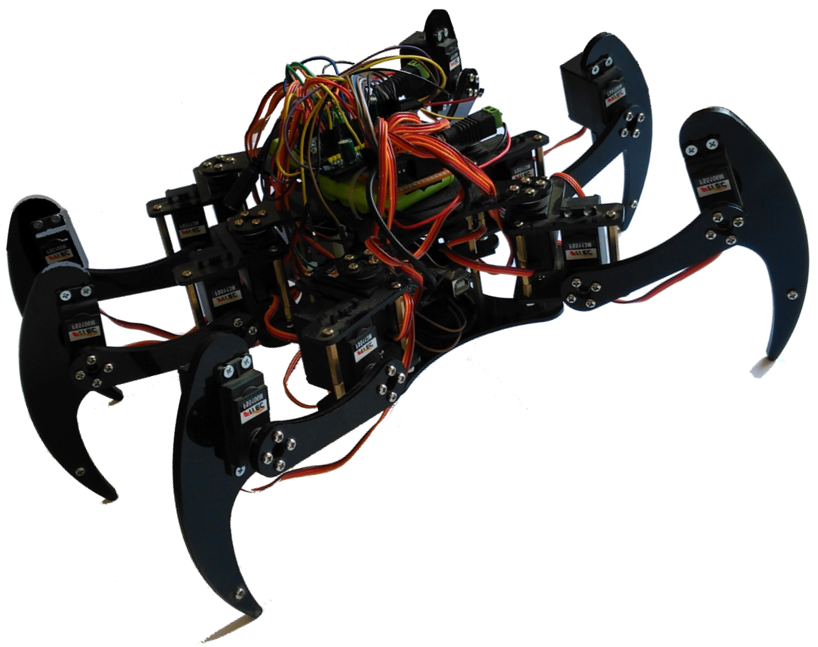
\includegraphics[width =0.8\textwidth]{Fig12}
    \caption{ A sex-legged walking robot.}
    \label{fig1}
\end{figure}

One of the interesting features of hexapod robots such as our ZagHexa (shown in Fig.\ref{fig1}) is that they can climb over obstacles larger than the equivalent sized wheeled or trucked vehicle. In fact, the use of wheels or crawlers limits the size of the obstacle that can be climbed to half the diameter of the wheels. On the contrary, legged robots can overcome obstacles that are comparable with the size of the machine leg\cite{2}. Hexapod walking robots also benefit from a lower impact on the terrain and have greater mobility in natural surroundings. This is especially important in dangerous environments like mine fields, or where it is essential to keep the terrain largely undisturbed for scientific reasons \cite{3}. \\

Hexapod legged robots have been used in exploration of remote locations and hostile environments such as seabed \cite{4}, in space or on planets \cite{5,6}  in nuclear power stations \cite{7}, and in search and rescue operations\cite{8}. Beyond this type of application, hexapod walking vehicles can also be used in a wide variety of tasks such as forests harvesting, in aid to humans in the transport of cargo, as service robots and entertainment. Development of hexapods is increasingly robust in the military sector. Armies all over the world are exploring ways of using hexapods to detect land mines, traverse rocky, unstable terrain, and carry out simple delivery missions in danger zones.

\section{History} 
Robots inspired by insects and other animals have previously been designed with physical antennae and tactile sensors to navigate their environment, as in the work by Brooks (1989) \cite{20,22}, Cowan et al. (2005), Hartmann (2001) \cite{27} and Lee et al. (2008) \cite{10}; the last three works employed the use of a single tactile element rather than a pair \cite{13}.
Because of their extreme mobility and agile adaptability to irregular terrain, insects have long been an inspiration for the designers of mobile and legged robots \cite{11,14}. Early hexapod robots such as Genghis and later creations such as Tarry implemented insect-like mobility based on observations of insect behaviors. The inter- leg coordination system developed by Holk Cruse \cite{30,23}  has been widely implemented   in legged hexapods and its basis is in behavioral experiments that qualitatively analyzed insect walking behaviors \cite{18}.

\subsection{Early Designs}
The first hexapods can be identified as robots based on a rigidly predetermined motion so that
an adaptation to the ground was not possible. Early researches in the 1950s were focused on assigning the motion control completely by a human operator manually\cite{11h}. 
\begin{figure}[h]
    \centering
    \begin{tabular}{ l l }
        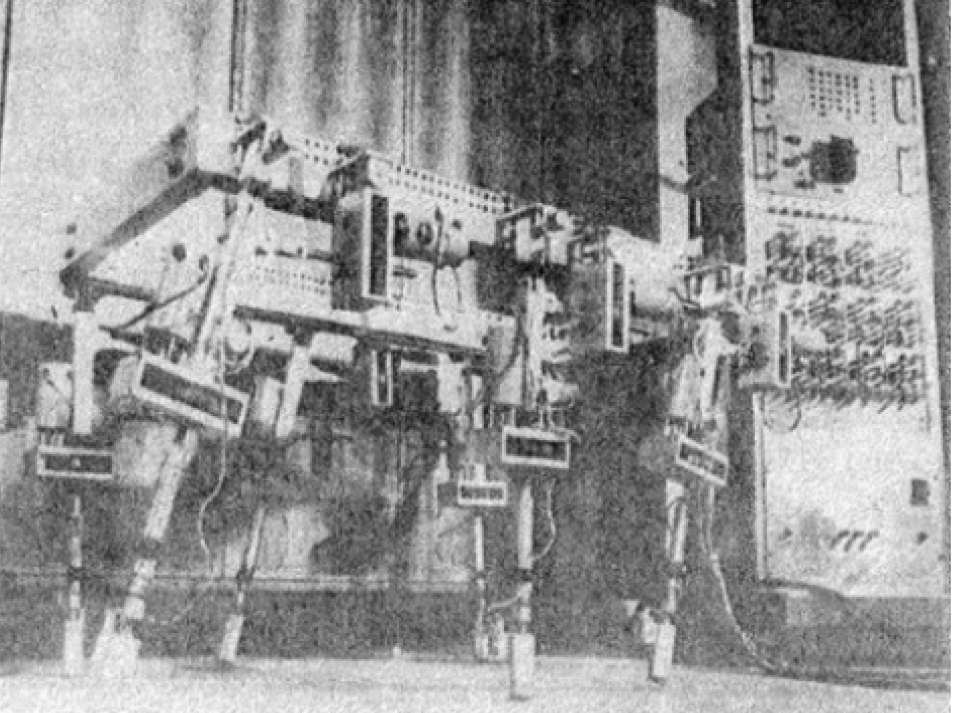
\includegraphics[width =.45\textwidth]{2_a} & 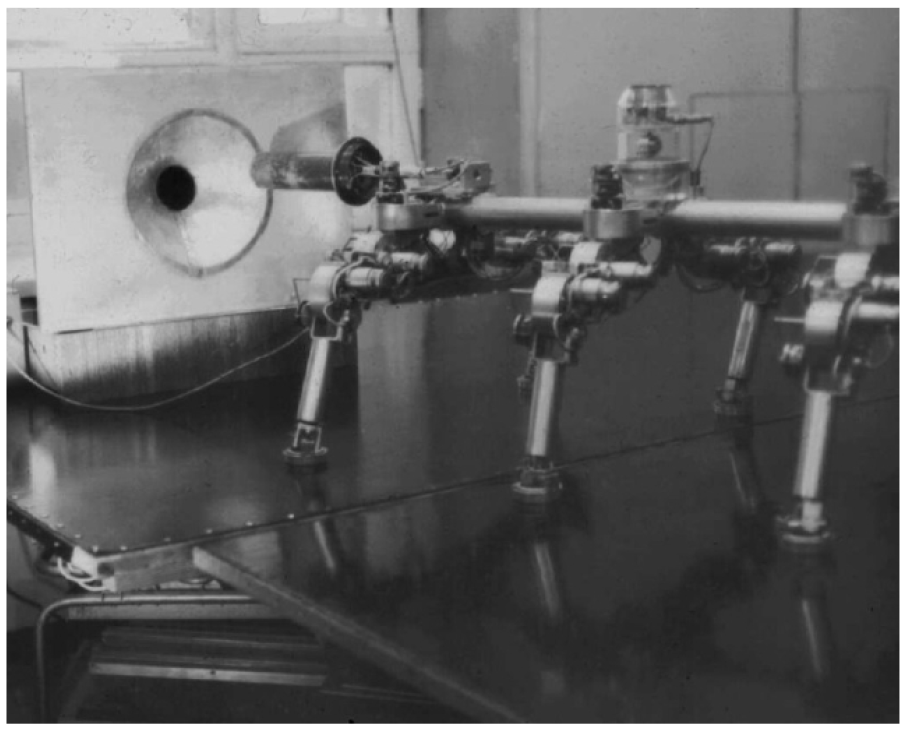
\includegraphics[width =.42\textwidth]{2_b} \\ 
        \hspace{3.5cm}(a) & \hspace{3.3cm}(b)\\
        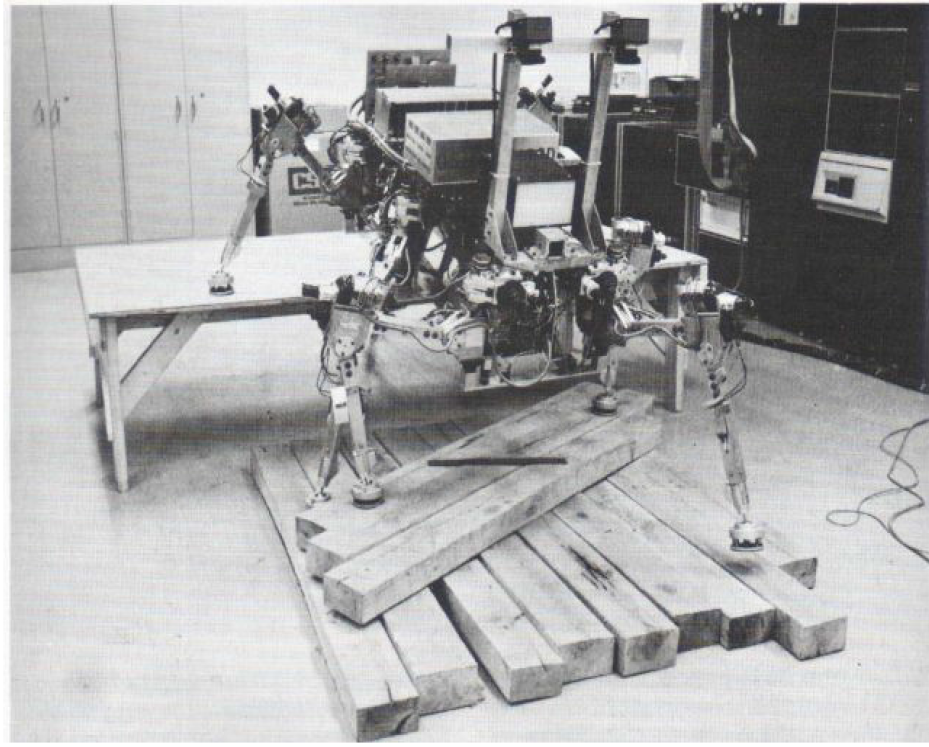
\includegraphics[width =.45\textwidth]{2_c} & \hspace{2cm} 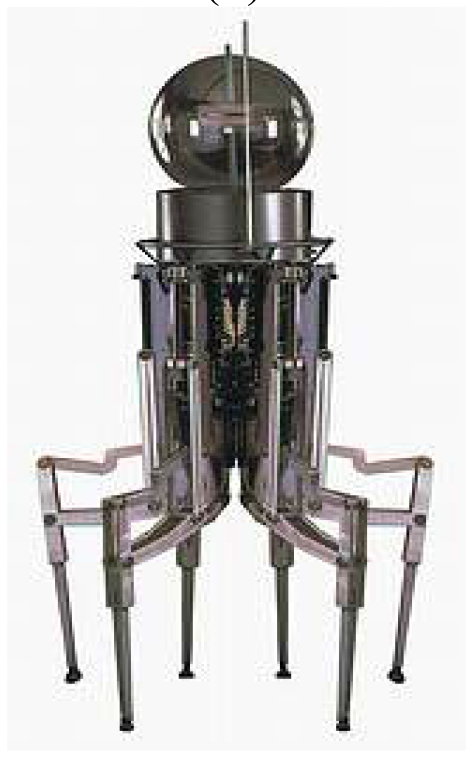
\includegraphics[width =.23\textwidth]{2_d} \\ 
        \hspace{3.5cm}(c) & \hspace{3.3cm}(d)\\
    \end{tabular}
    \caption{Early hexapod design: (a) University of Rome’s hexapod; (b) MASHA hexapod; (c) OSU hexapod; (d) ODEX I hexapod.}
    \label{fig2}
\end{figure}

One of the first successful hexapod robot was constructed at University of Rome in 1972 (Fig.\ref{fig2}a) as a computer-controlled walking machine with electric drives\cite{12h}. In the middle 70s, at the Russian Academy of Sciences in Moscow, a six-legged walking machine was developed with a mathematical model of motion control. It was equipped with a laser scanning range finder and was connected with a two-computer control system \cite{13h}. In 1976, Masha hexapod walking robot was designed at Moscow State University (Fig.\ref{fig2}b). The robot had a tubular axial chassis, articulated legs with three DoFs \cite{14h}. The hexapod was able to negotiate obstacles using contact on the feet and a proximity sensor. Ohio State University in 1977 developed a six-legged insect-like robot system called “OSU Hexapod” \cite{15h}. This hexapod was kept tethered and was made to walk short distances over obstacles (Fig.\ref{fig2}c).
In 1984, Odetic Inc., California, USA, developed Odex I \cite{17h}, a six-legged radially symmetric hexapod robot which used an onboard computer to play back pre-programmed motions (Fig.\ref{fig2}d).


\subsection{Recent Developments}
The two last decades have been characterized by a rapid development of control systems technology. Hexapod robots were equipped with various sensing systems. Artificial Intelligence systems were widely applied to the analysis of environment and motion of robots on a complex surface. A series of bio inspired robots was developed at Case Western Reserve University (USA) at the end the 90s, such as, for example, Robot III that had a total of 24 DoFs. Robot III architecture was based on the structure of cockroach, trying to imitate their behavior \cite{25h}. In particular, each rear leg had three DoFs, each middle leg four DoFs and each front leg five DoFs. Similarly, Biobot was a biomimetic robot physically modeled as the American cockroach (Periplaneta Americana) and powered by pressurized air \cite{26h}. This hexapod had a great speed and agility. \\
Each leg of the robot had three segments, corresponding to the three main segments of insect legs: coxa, femur, and tibia.
\begin{figure}[h]
    \centering
    \begin{tabular}{ l l }
        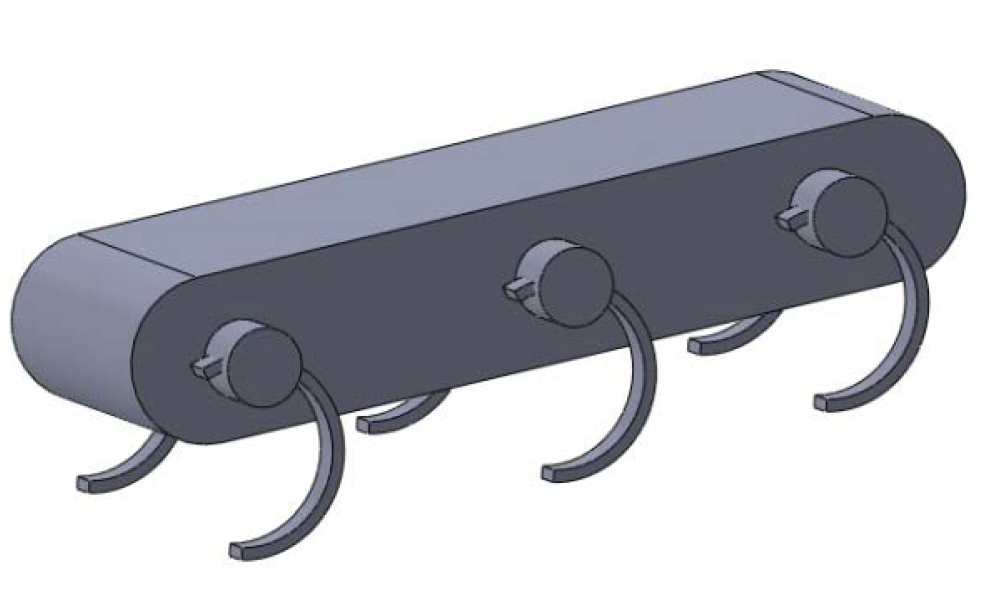
\includegraphics[width =0.45\textwidth,height=0.2\textheight]{3_a} & 
        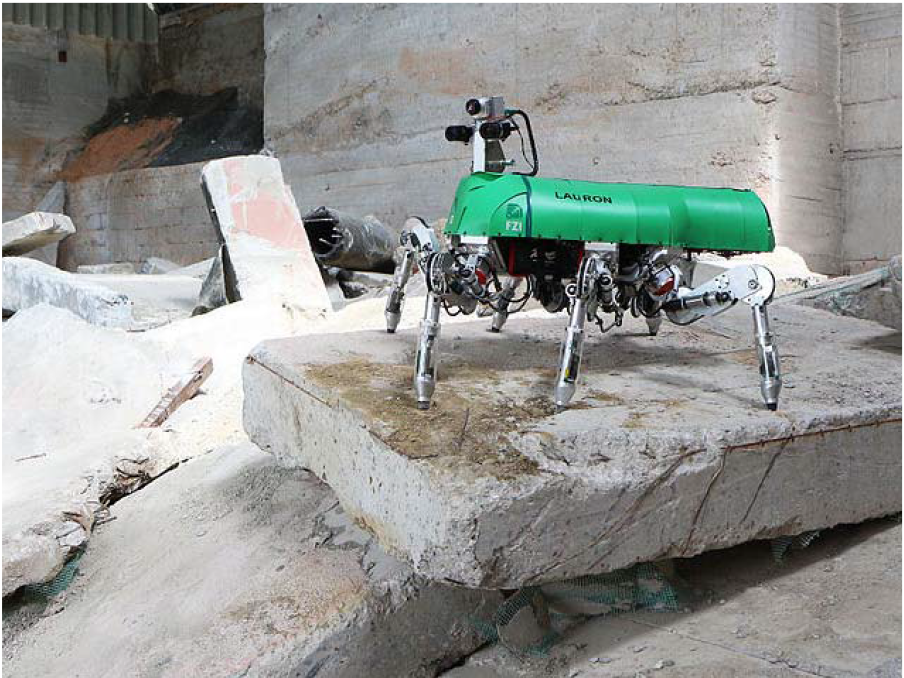
\includegraphics[width =0.45\textwidth,height=0.2\textheight]{3_b} \\ 
        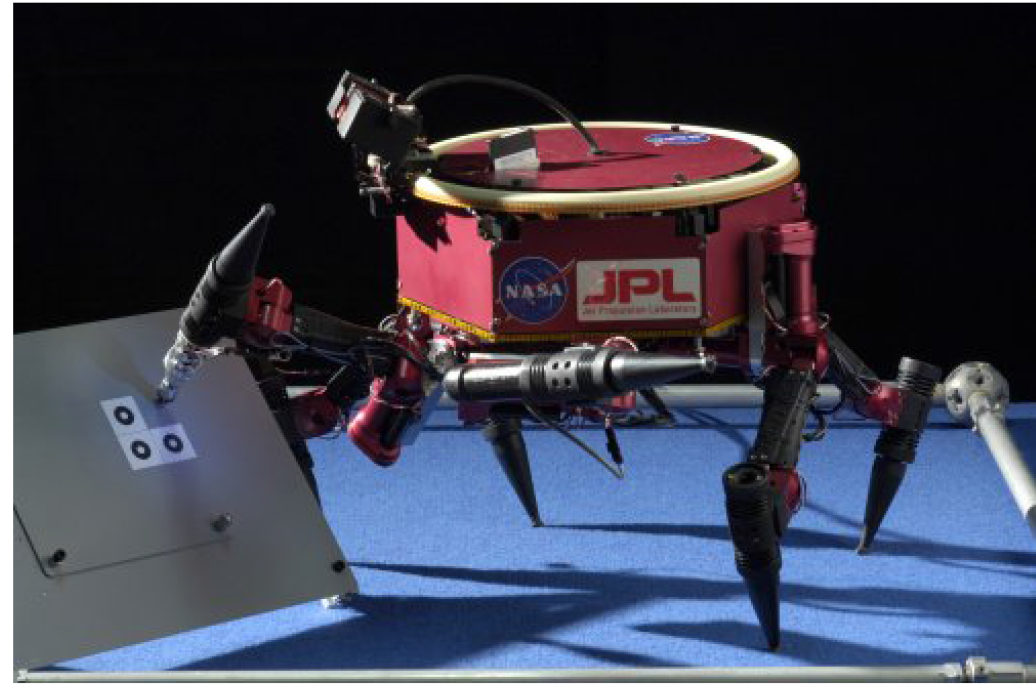
\includegraphics[width =0.45\textwidth,height=0.2\textheight]{3_c} & 
        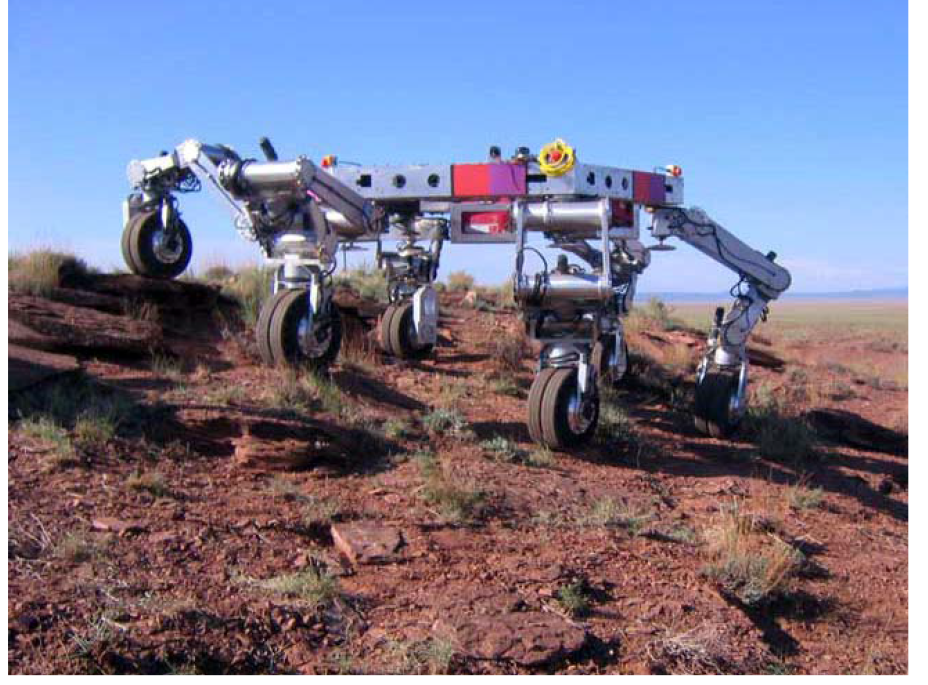
\includegraphics[width =0.45\textwidth,height=0.2\textheight]{3_d} \\ 
    \end{tabular}
    \caption{Some Example on recent developments in hexapod design}
    \label{fig3}
\end{figure}


%\input{chapters/stateOfArt}
%%%%%%%%%%%%%%%%%%%%%%%%%%%%%%%%%%%%%%%%%%%%%%%%%%%%%%%%%%%%%%%%%%%%%%%%%%%%%%%

\setchapterpreamble[o]{%
\dictum[Joseph Addison, \textit{(English essayist, poet, and politician, 1672--1719), Spectator, No. 253}]{% source: http://todayinsci.com/A/Addison_Joseph/AddisonJoseph-Quotations.htm
``It is impossible for us, who live in the latter ages of the world, to make observations in criticism, morality, or in any art or science, which have not been touched upon by others. We have little else left us but to represent the common sense of mankind in more strong, more beautiful, or more uncommon lights.''}\vspace{0.1em}}

\chapter{Design Considerations}\label{ch:design} %and Related Work
%Hardware design
In this chapter we will walk through the hardware design of our hexapod including both mechanical and electronic parts

\section{Design consideration}
Designing hexapod legged robots is far from trivial. A very numerous and a wide range of possibilities exist to design a hexapod. Designers must take several decisions which influence the operation and technical features. Some of the most important design issues and constraints according to \cite{48h} can be outlined as:

\begin{itemize}
	\item The mechanical structure of robot body.
	\item Leg architecture.
	\item Max sizes.
	\item Actuators and drive mechanisms.
	\item Control architecture.
	\item Power supply.
	\item Walking gaits and speed.
	\item Obstacle avoidance capability.
	\item Payload.
	\item Autonomy.
	\item Operation features.
	\item Cost.
\end{itemize}

The above mentioned design issues and constraints can be classified as design input (or key	features) and design output (or main design characteristics) as shown in the scheme of \ref{GD}.

\begin{figure}[H]		
	\centering
	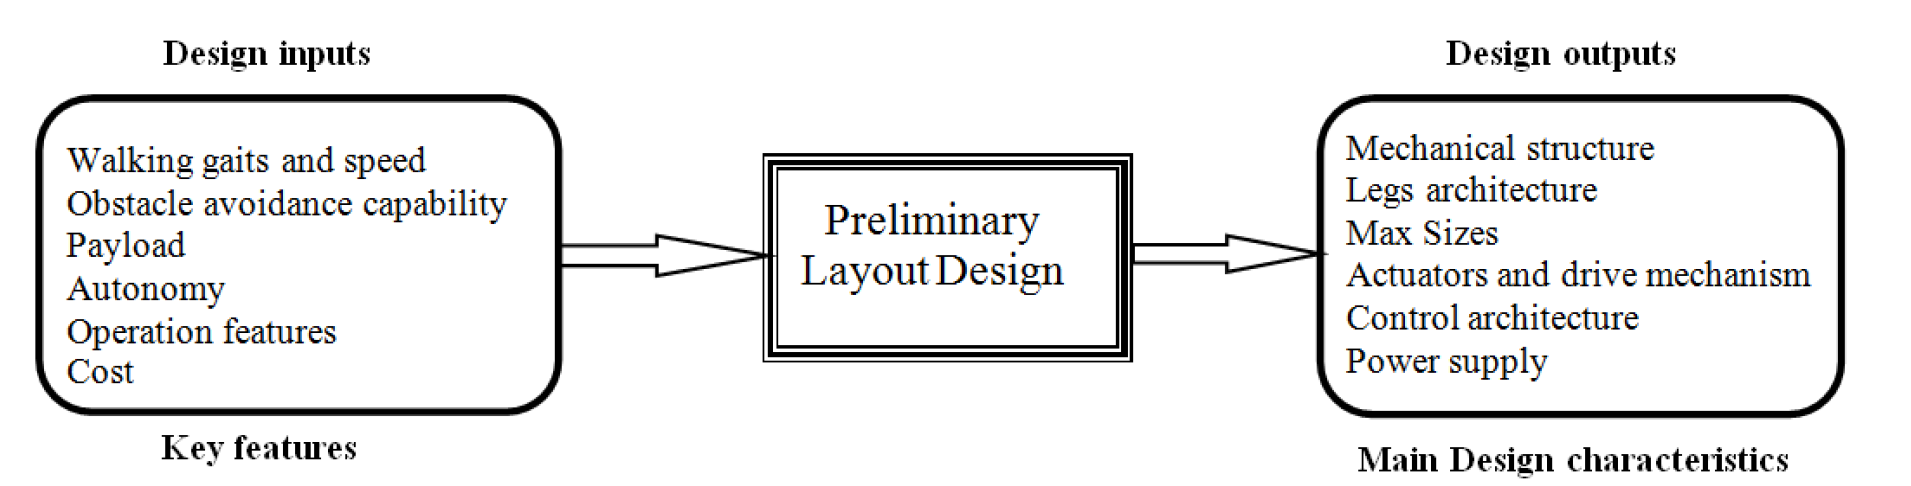
\includegraphics[width =.8\textwidth]{GD}
    \caption{ A scheme for preliminary layout design of hexapod walking robots.}
	\label{GD}
\end{figure}

\section{Hardware overview}
ZagHexa is a hexapod robot with 18 DOFs (three degrees of freedom (DOF) for each leg), it can walk in any direction (translation), or turn in place (rotation), or any combination of the two. The leg lift and ride height is adjustable as well. The robot uses a distributed walking control system based on the neurobiology of insects, stepping in the sagittal plane to angled stepping, which then induces turning in the robot.
It is an integrated multi-legged walking robot based on de-facto standard Robotic Operating System (ROS) that employs novel and different walking patterns.
Our robot is teleoperated using hand-held devices such as a smart phone or tablet or a wireless joystick (see Fig.\ref{fig4}). Furthermore, it has its own navigation system and a camera for instant video recording and streaming.
The power to the entire system is supplied through two 5 volts NiMH batteries. There is an additional power bank to power up the Raspberry Pi and other electronic components. 

\begin{figure}[H]
	\centering
	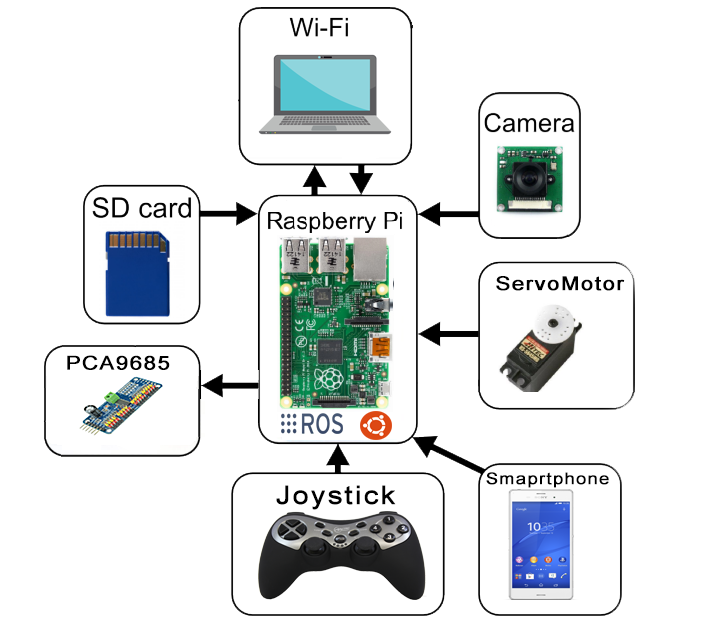
\includegraphics[width =.5\textwidth]{Fig2}
	\caption{ The electronic system of the robot.}
	\label{fig4}
\end{figure}

The final design of the ZagHexa robot constructed mainly with acrylic is shown in Fig.\ref{fig1}. ZagHexa body moves independently of its ground contact points. To make its center of gravity shift on a horizontal plane, forward/backward, and sideways moving functions are effective. These functions can also produce a smooth body movement independently of intermittent leg traveling. The robot has been designed with three degrees of freedom in the front, middle and rear legs respectively. The physical specifications are given in Table 2.
\begin{center}
\begin{tabular}{|c|c|}
    \hline
    Parameter       &       Description        \\ \hline
    Length         &           30cm           \\ \hline
    Width         &           27cm           \\ \hline
    Height         &           17cm           \\ \hline
    Weight         &           3Kg            \\ \hline
    Construction Material &                          \\ \hline
    Actuators       &     DC servo motors      \\ \hline
    Motion Control     & Servo Sequential Control \\ \hline
    Leg Stroke (Max)    &           6cm            \\ \hline
    Leg Lift (Max)     &           5cm            \\ \hline
\end{tabular}
\end{center}
\noindent
%Mechanical design
\section{Mechanical design}
\noindent In this section we will discuss the different designs of the robot including early ones as well as the final one.
\subsection{Micro ZagHexa}
We started by making a small hexapod with 18 micro servos to test our basic functions and walking algorithms. The basic parts of Micro ZagHexa is made of a 1 mm thick Aluminium sheet.

\begin{figure}[H]
	\centering
	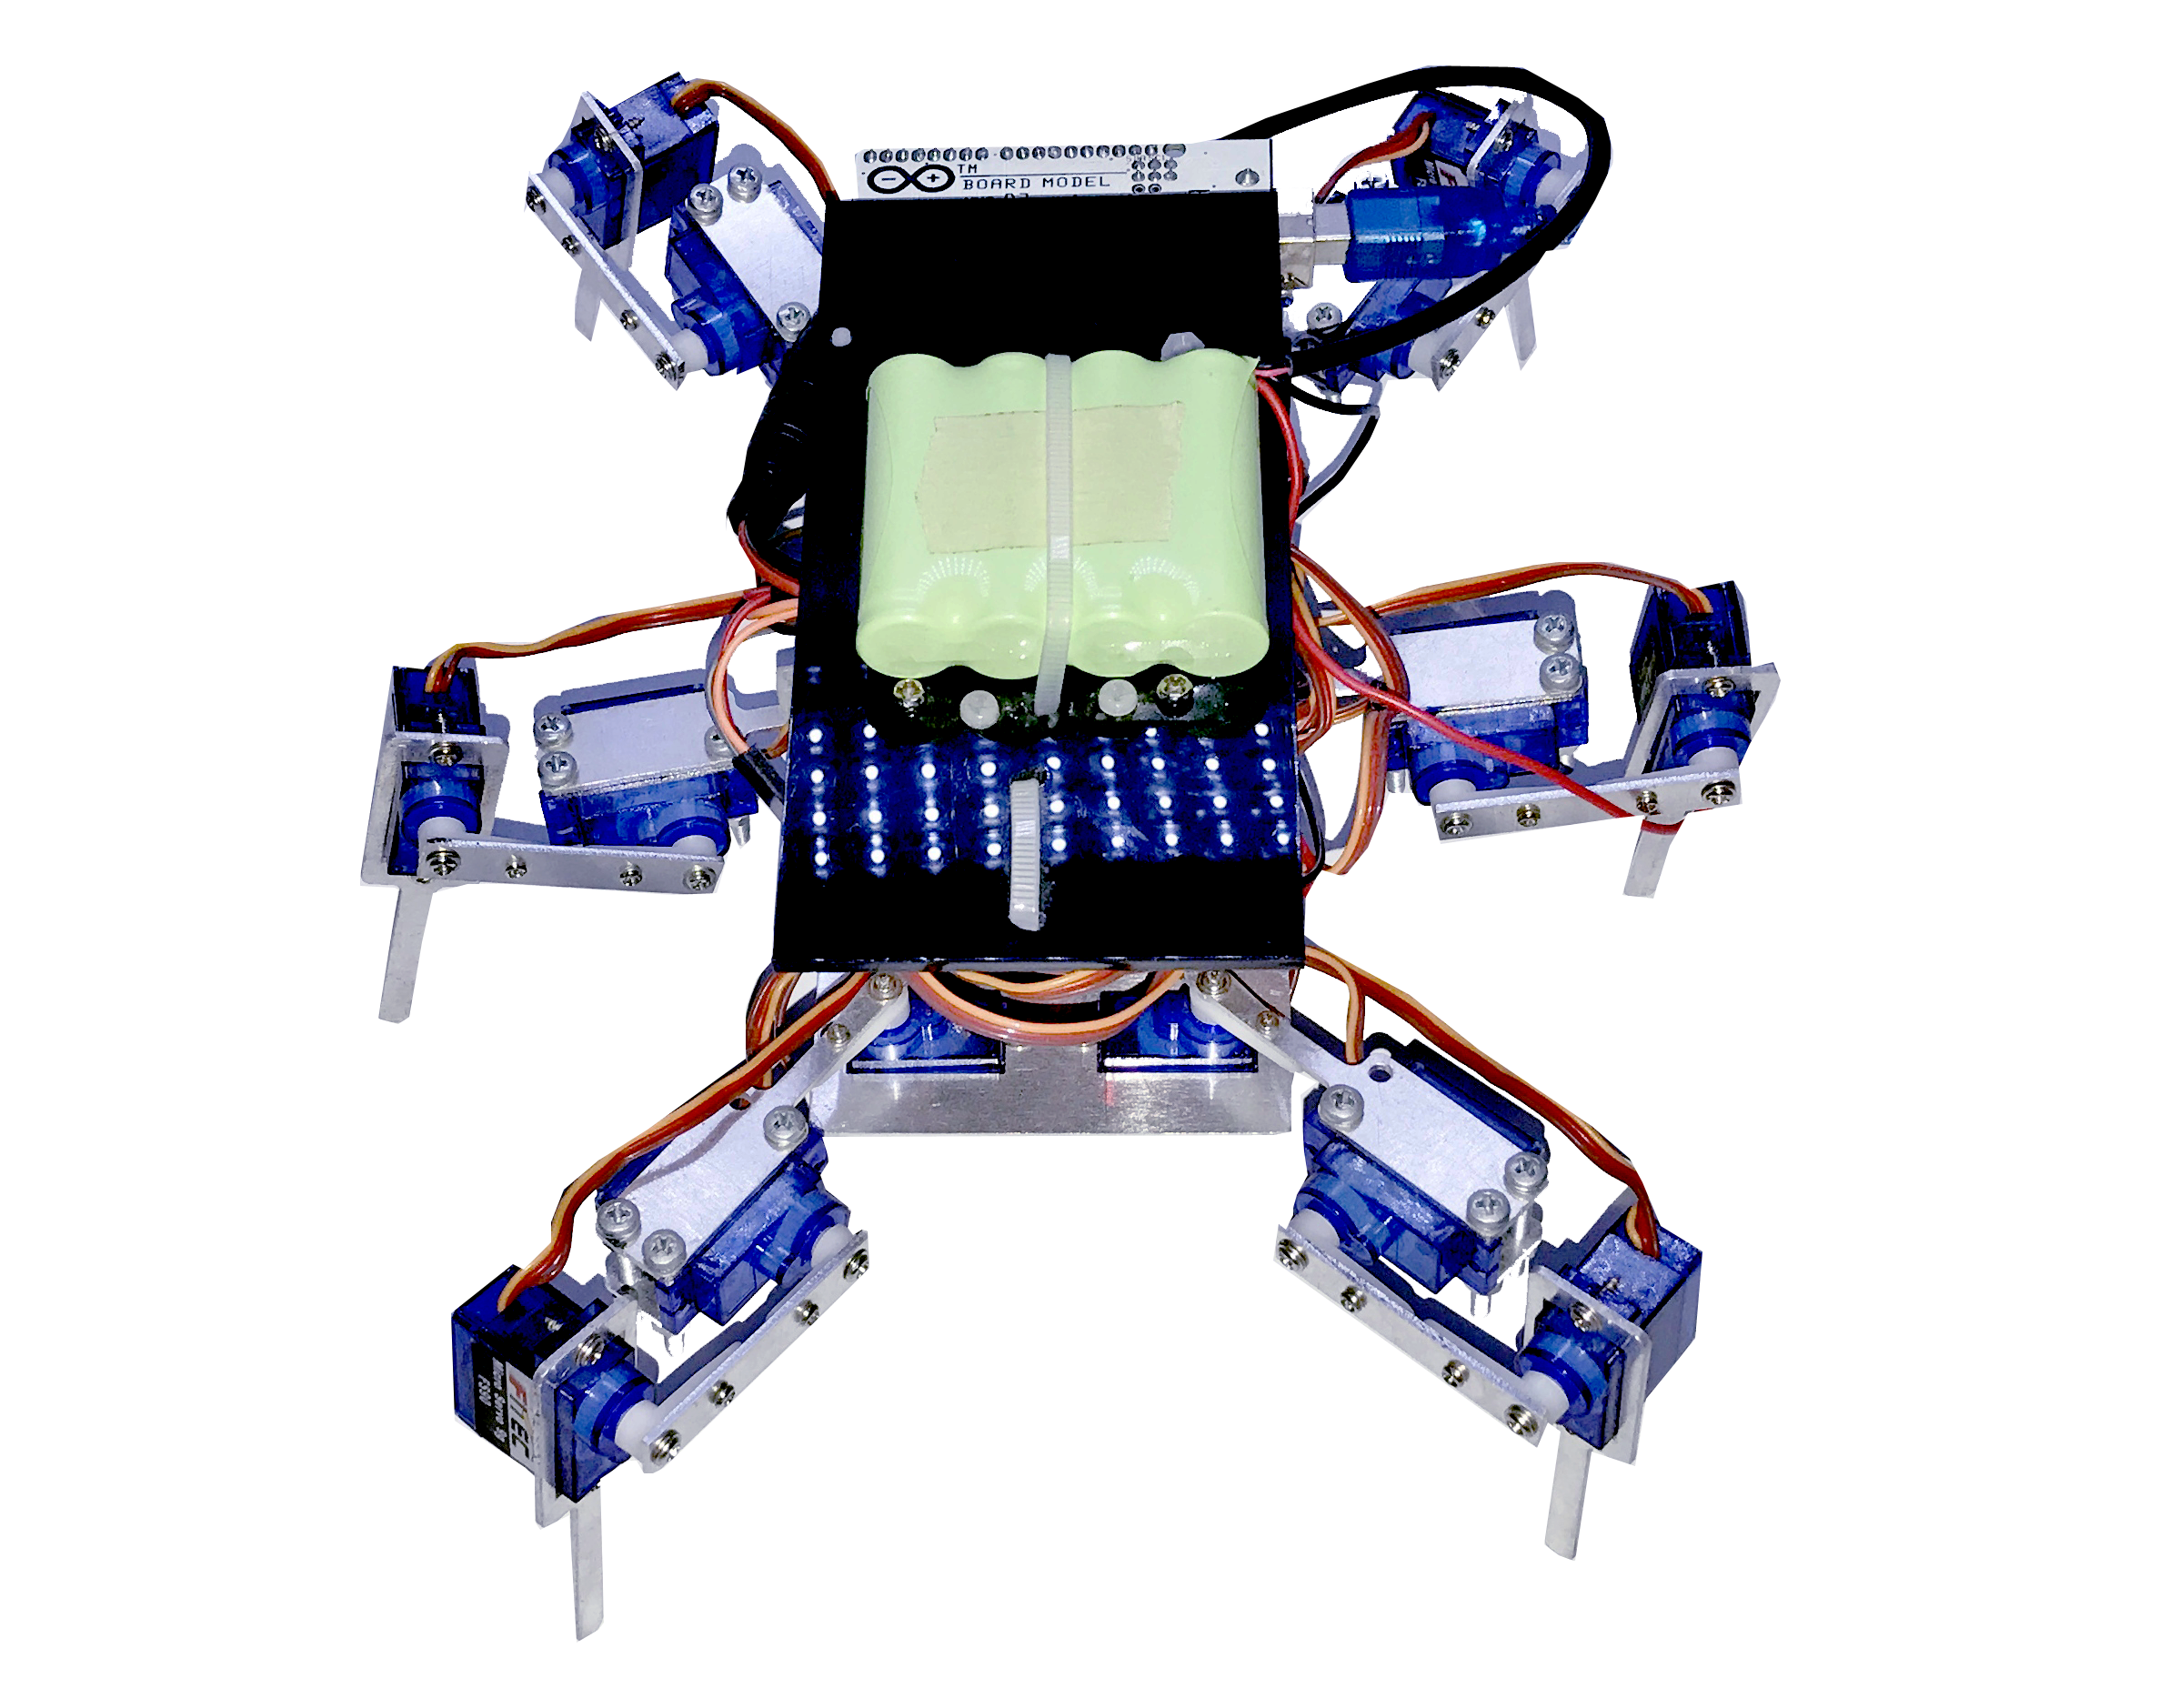
\includegraphics[width=5cm,height=5cm]{figures/uZagHexaFinal.png}
	\caption{Micro ZagHexa}
	\label{figure_i}
\end{figure}

\subsection{ZagHexa}
We moved to our next hexapod design and made it bigger and more natural looking with an articulate leg and body design. ZagHexa is made of 2.5 mm thick Acrylic. \ref{figure_} shows the CAD model of Zaghexa and \ref{figure_} shows it after being assembled.
%\begin{figure}[h]
%	\centering
%	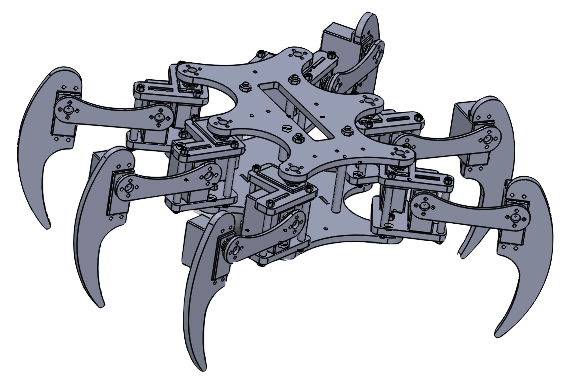
\includegraphics{figure_j}
%	\caption{CAD model of ZagHexa}
%	\label{figure_j}
%\end{figure}
\begin{figure}[H]
	\centering
	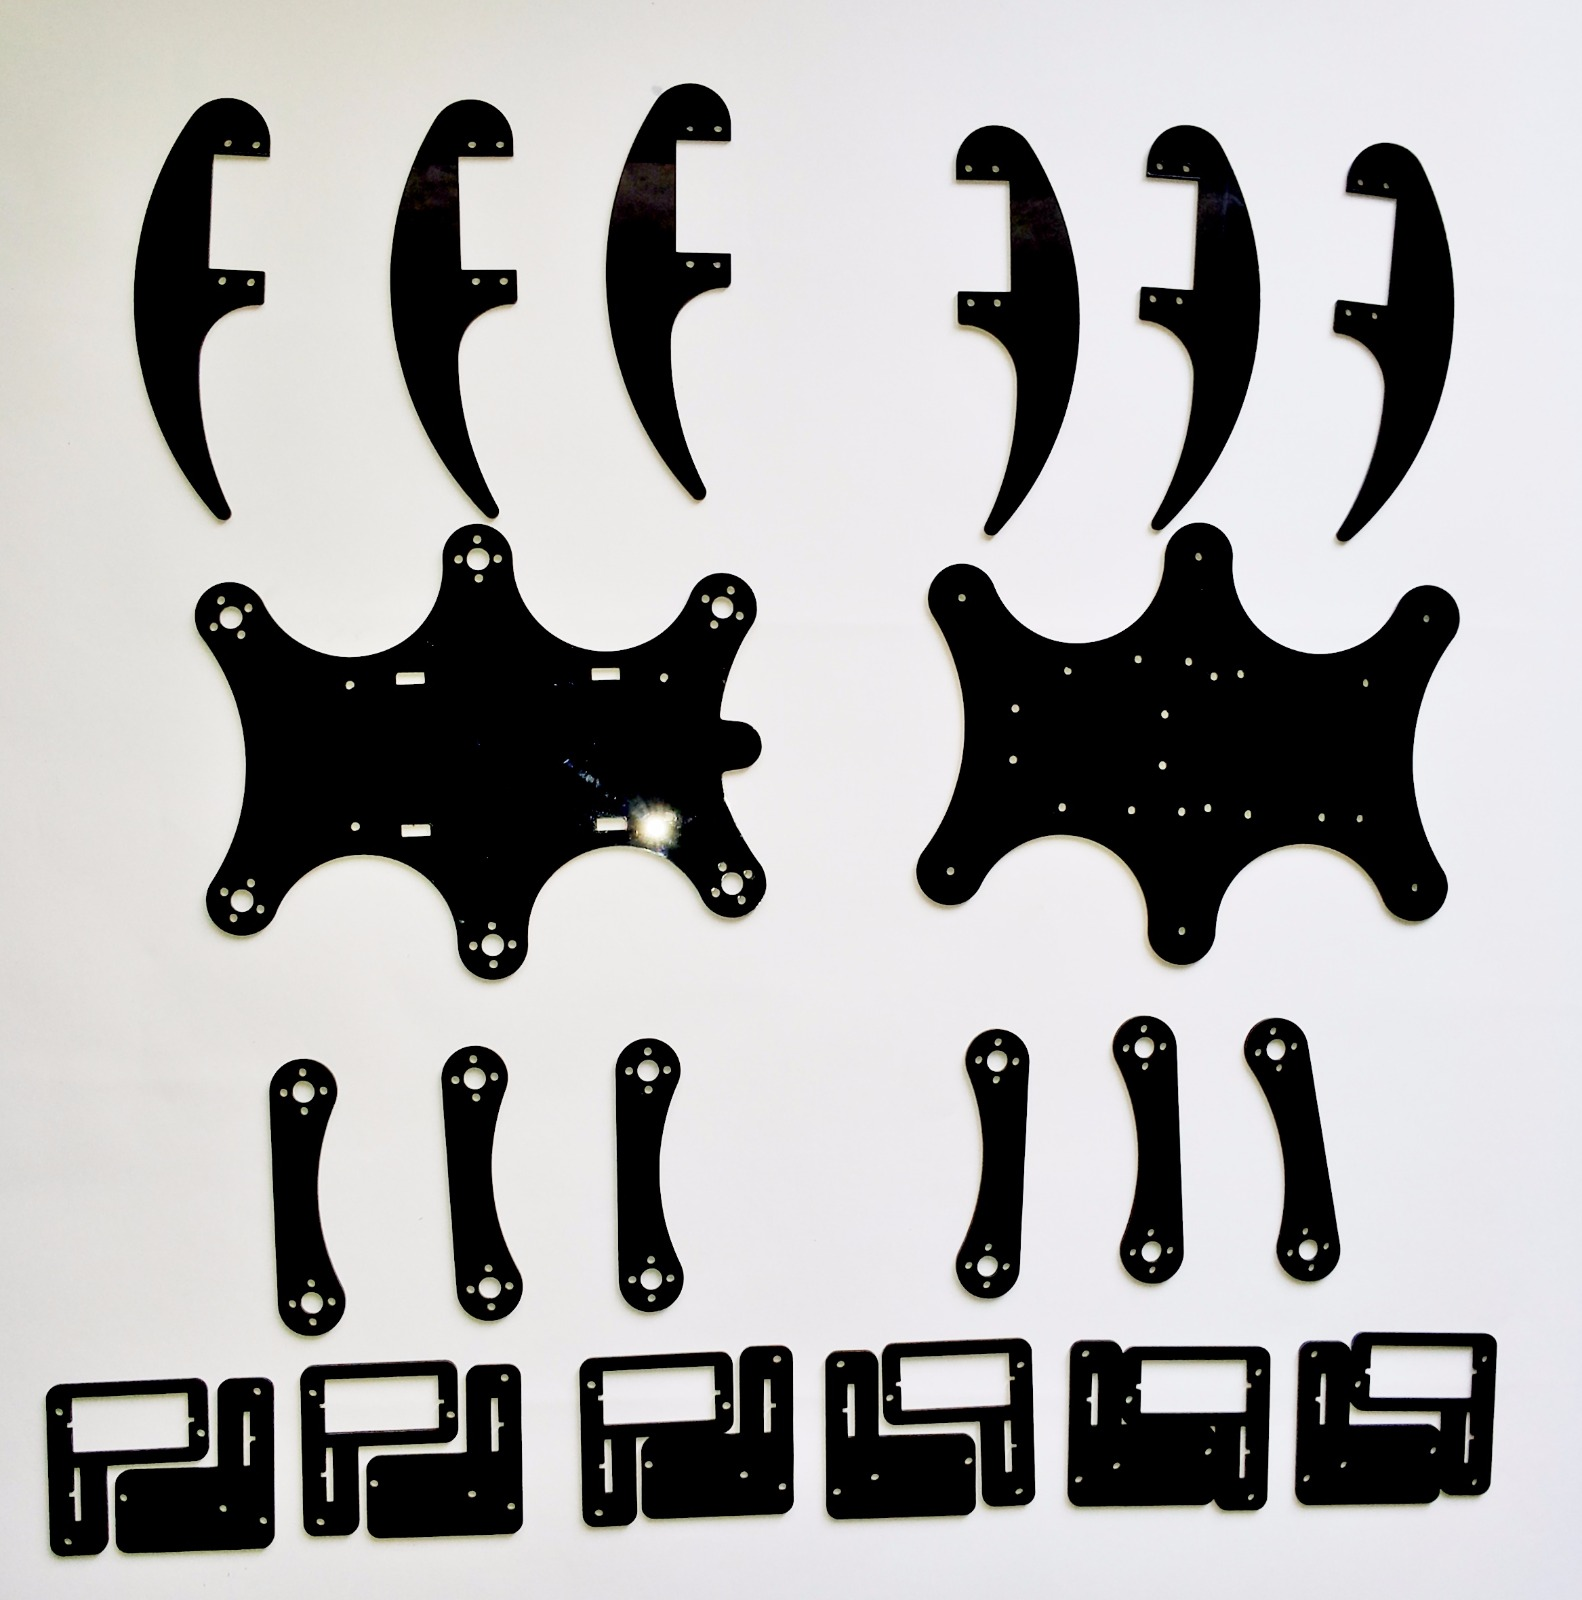
\includegraphics[width=10cm,height=11cm]{figure_k}
	\caption{ZagHexa during assembling}
	\label{figure_k}
\end{figure}
\begin{figure}[H]
	\centering
   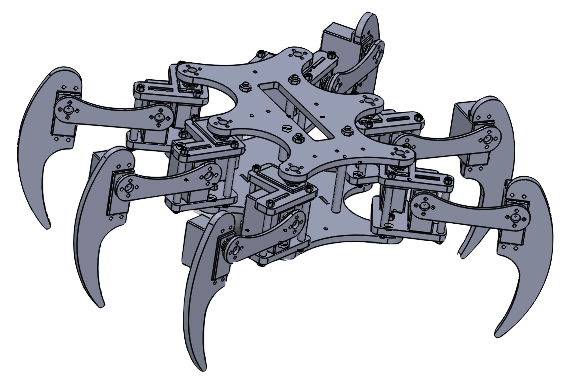
\includegraphics[width=0.45\textwidth]{figure_j}
	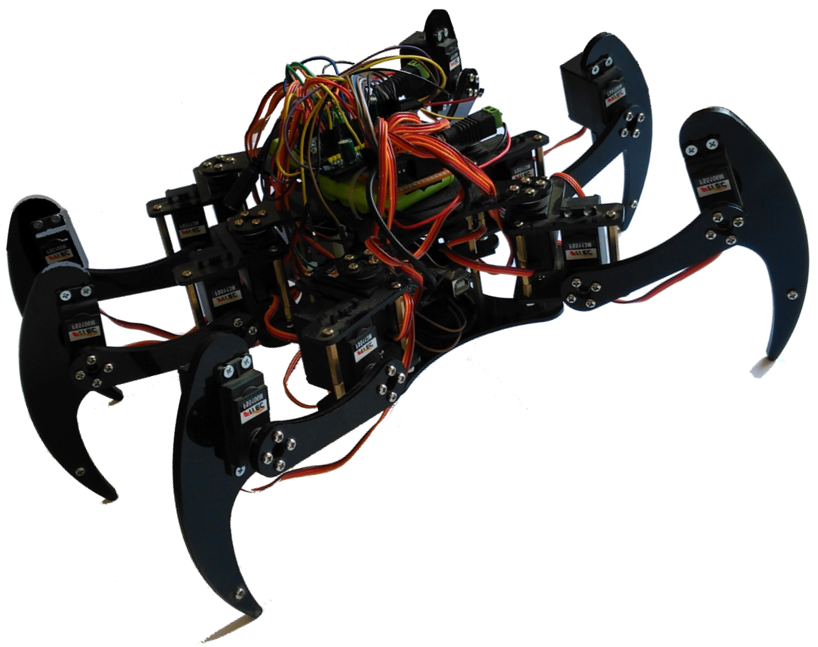
\includegraphics[width=0.45\textwidth]{Fig12}
	\caption{CAD model (left) and assembled ZagHexa (right)}
	\label{figure_l}
\end{figure}

\subsection{Giant ZagHexa}
Lastly, we made the giant version of our hexapod. It is made of a double layer 1 mm thick Aluminium sheet. The CAD model of Giant ZagHexa is shown in \ref{figure_m} and \ref{figure_o} shows it after assembling.
\begin{figure}[H]
	\centering
	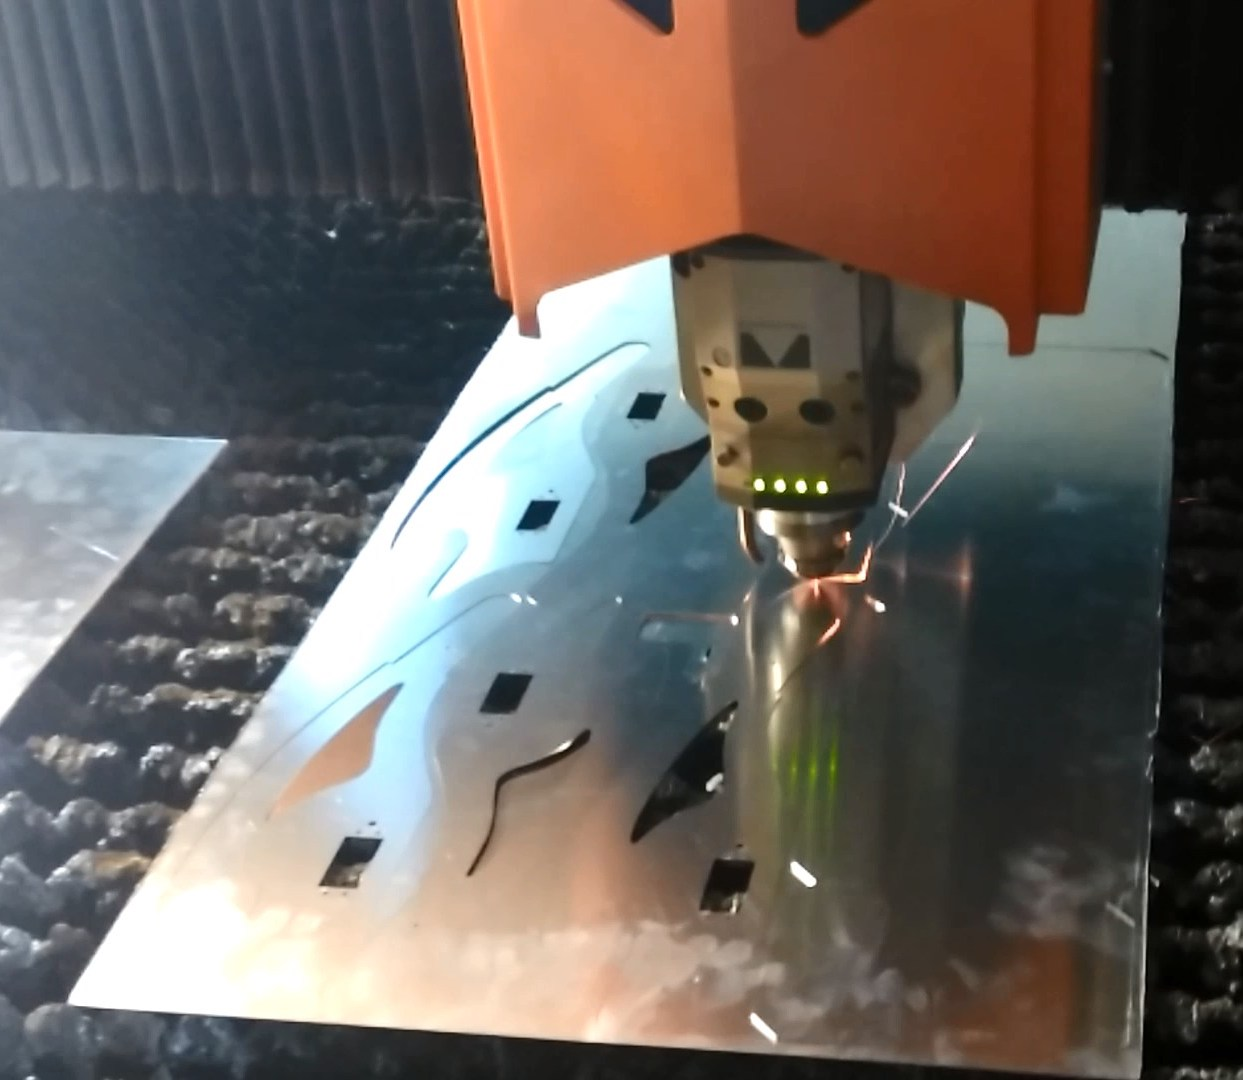
\includegraphics[width=0.7\textwidth]{figure_n}
	\caption{Giant ZagHexa during laser cutting}
	\label{figure_n}
\end{figure}
\begin{figure}[H]
	\centering
    	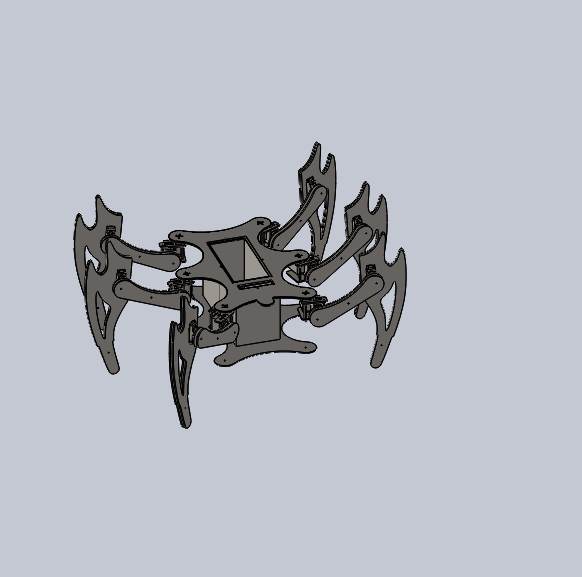
\includegraphics[width=0.45\textwidth]{figure_m}
	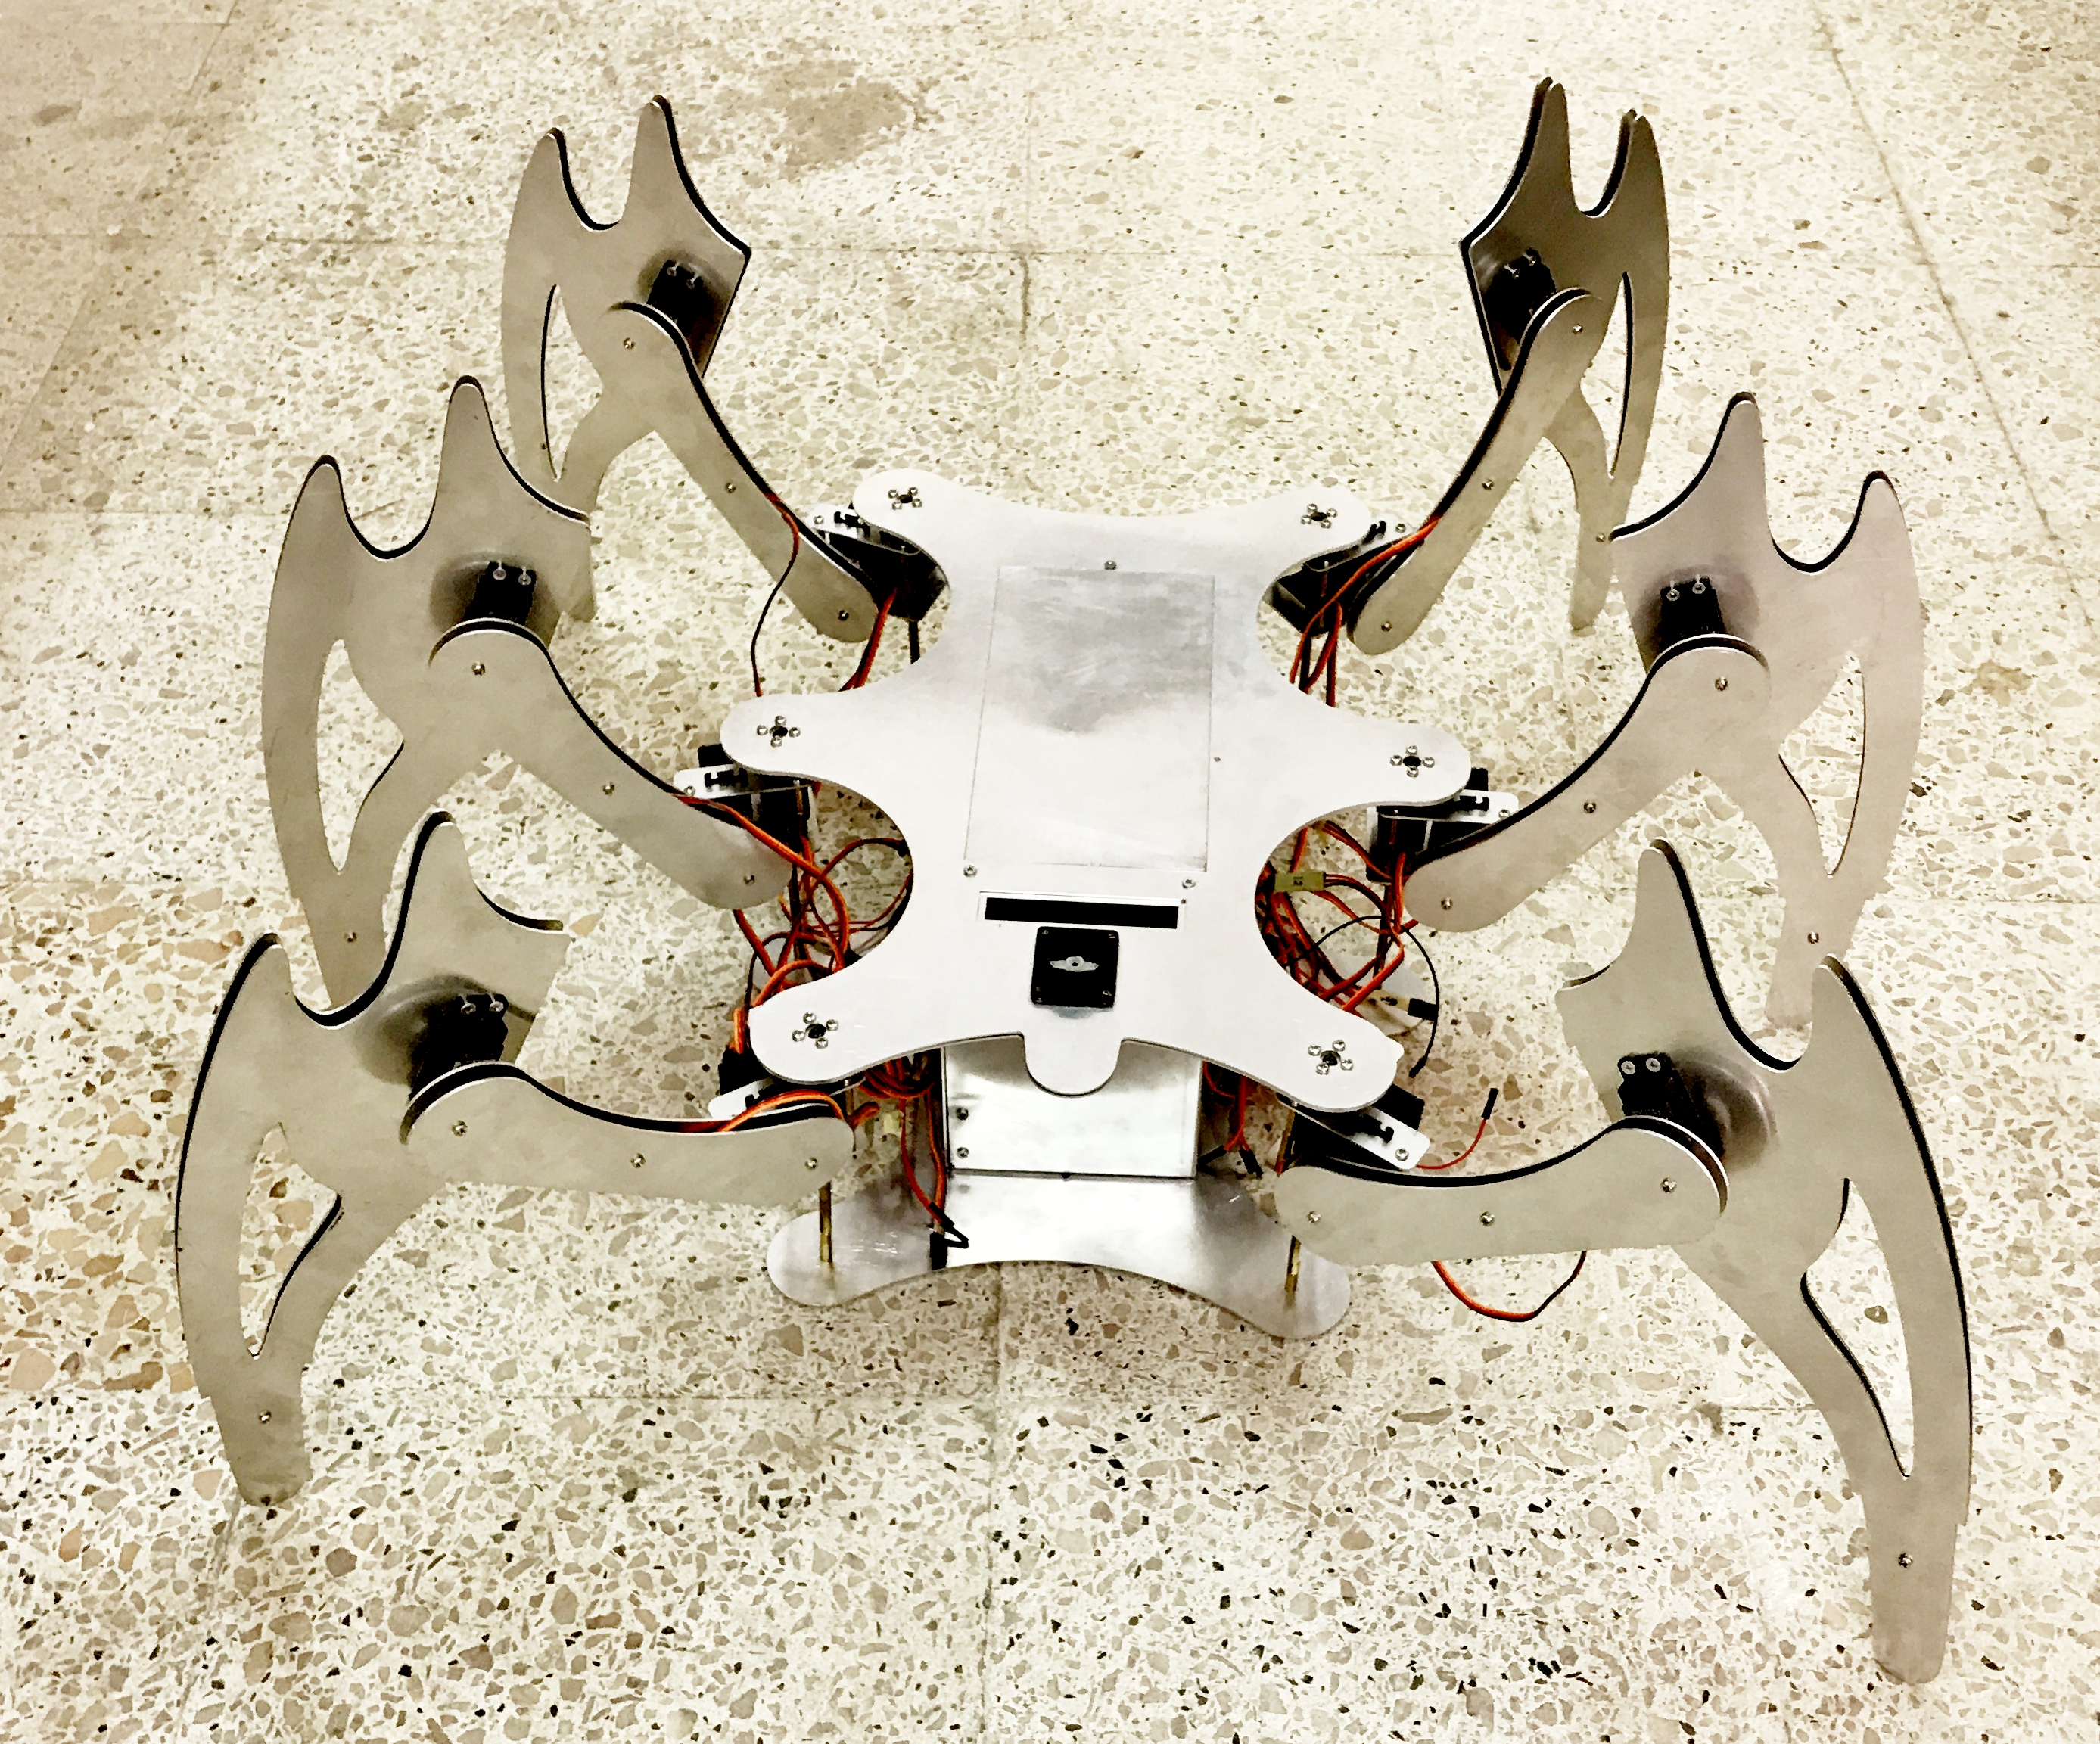
\includegraphics[width=0.45\textwidth]{figure_o}
	\caption{CAD model (left) and assembled Giant ZagHexa (right)}
	\label{figure_o}
\end{figure}


The giant ZagHexa was a little disappointing as servo motors were not strong enough to drive our hexapod. We tried to make the chassis lighter but that did not solve the problem completely. It still have stability issues.

%Electronics
\section{Electronics}
In this section we will talk about the electronic components we have been using through the whole project.
\subsection{Adafruit PCA9685}
Firstly, we used the Adafruit PCA9685 servo controller shown in \ref{figure_i} and \ref{figure_j}. Although driving servo motors with the Arduino Servo library is pretty easy, each one consumes a precious pin - not to mention some Arduino processing power.  The Adafruit 16-Channel 12-bit PWM/Servo Driver will drive up to 16 servos over I2C with only 2 pins.  The on-board PWM controller will drive all 16 channels simultaneously with no additional Arduino processing overhead.  Moreover, we can chain up to 62 of them to control up to 992 servos - all with the same 2 pins!
\begin{figure}[H]
	\centering
	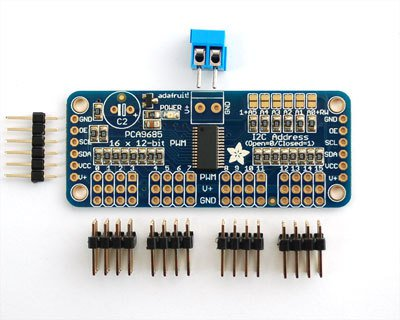
\includegraphics{figure_i}
	\caption{Adafruit PCA9685}
	\label{figure_i}
\end{figure}
\begin{figure}[H]
	\centering
	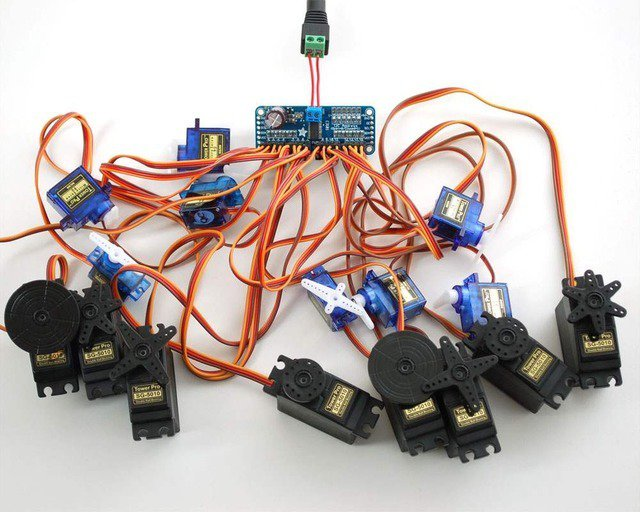
\includegraphics[width=14cm,height=10cm]{figure_p}
	\caption{Adafruit PCA9685 wiring}
	\label{figure_p}
\end{figure}
\subsection{Servo Motors}
We used 18 servo motors of different sizes as actuators. A 7 kg.cm servo motor is used to drive the tibia part as well as the coxa. The motor that will lift the whole leg should be much stronger so we used a 13 kg.cm servo. That's it, we have 3 servo motors in each leg(3 DOFs): one for coxa and one for tibia and a stronger one for the femur.

\begin{figure}[H]
	\centering
	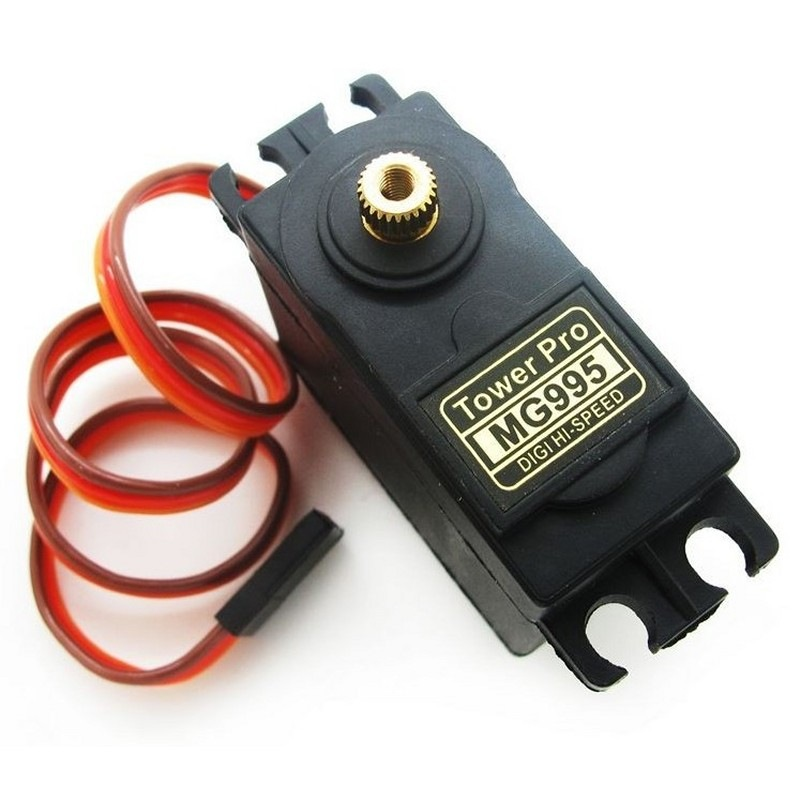
\includegraphics[width=10cm,height=5cm]{figure_q}
	\caption{13 kg.cm servo motor}
	\label{figure_q}
\end{figure}

\subsection{Playstaion joystick}
In earlier versions of ZagHexa, we used a wireless playstation 2 controller to teleoperate the hexapod. It communicates with the arduino through its uniqe via an SPI communication protocol.

\begin{figure}[H]
	\centering
	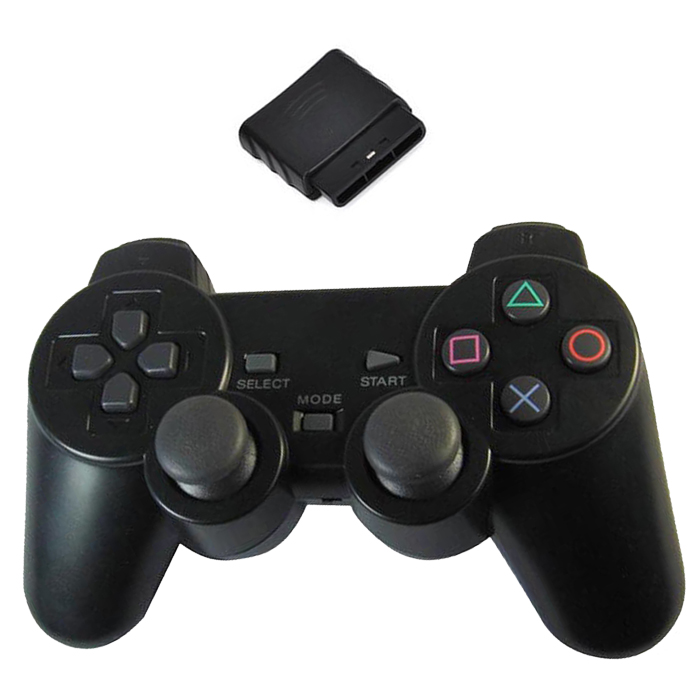
\includegraphics{figure_r}
	\caption{Playstaion 2 controller}
	\label{figure_r}
\end{figure}

\subsection{PS2/Serial converter}
A converter is used to keep the communication between the joystick and the controller happens serially so it well be easier to handle.

\begin{figure}[H]
	\centering
	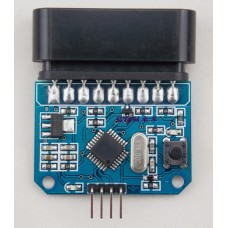
\includegraphics[width=6cm,height=8cm]{figure_s}
	\caption{PS2/Serial adapter}
	\label{figure_s}
\end{figure}

\subsection{Arduion Mega}
Later, we use an Arduino Mega in replacement of the PCA 9685 servo controller to send PWM signals to each servo motor. The reason why we moved our work from the servo controller to the Arduino Mega is that the servo controller can NOT withstand voltage above 6 Volts nor current above 5 Amps.

\begin{figure}[H]
	\centering
	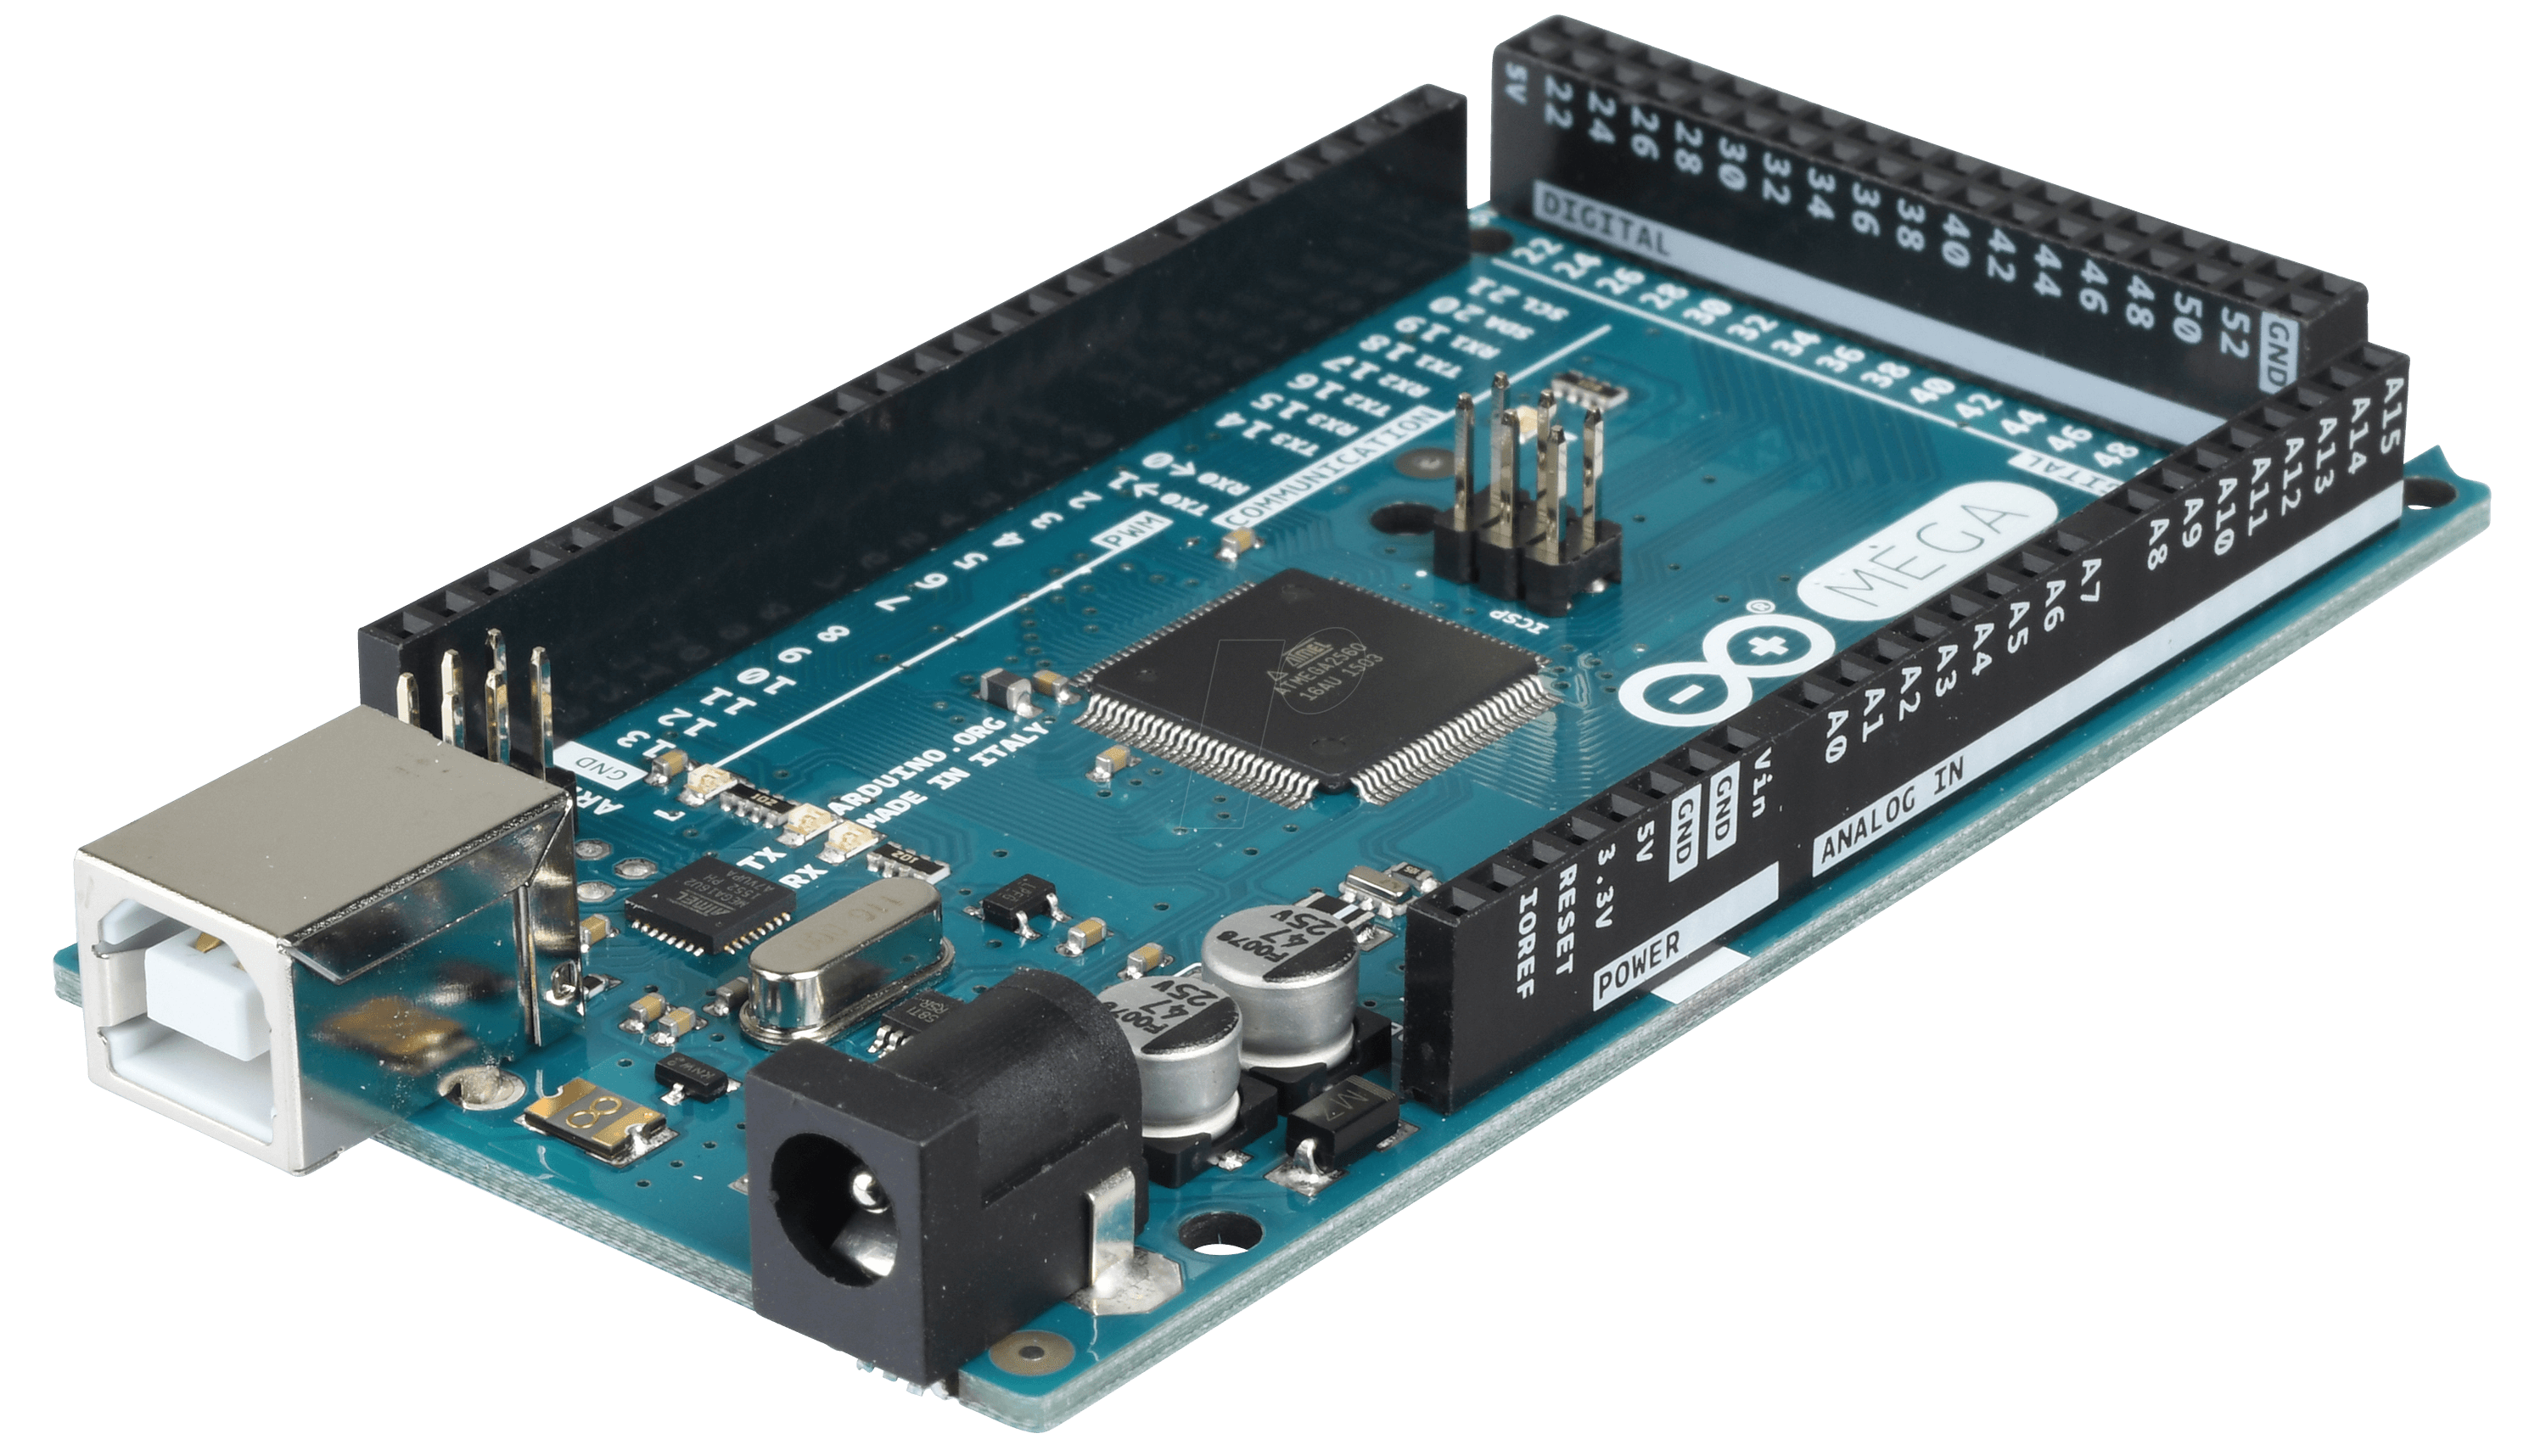
\includegraphics[width=14cm,height=10cm]{figure_t}
	\caption{Arduino Mega 25600}
	\label{figure_t}
\end{figure}

\subsection{Servo interface}
We want to make a servo interface with the arduino mega and that would make installing the servos so easy without making a mess. In theory we could use 48 servos on a Mega board, but we only soldered 18 servo ports, just to keep wires tidy and compact.

\begin{figure}[H]
	\centering
	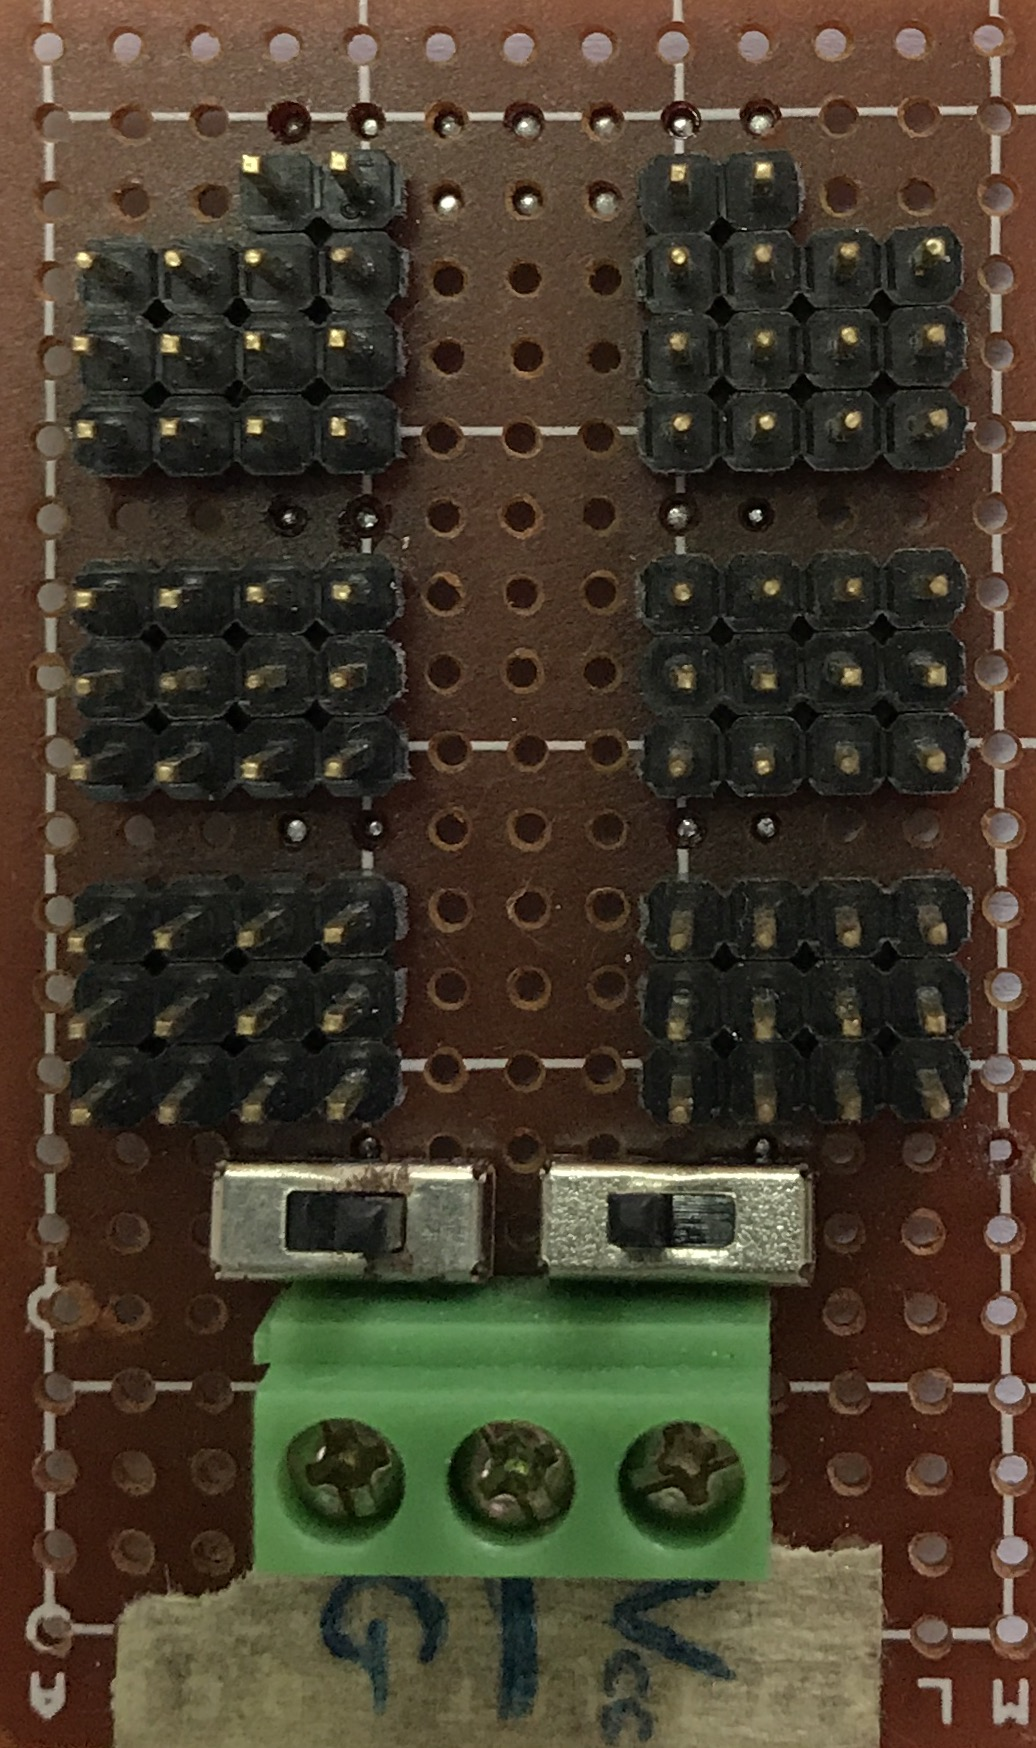
\includegraphics[width=4cm,height=6cm]{figure_u}
	\caption{Servo interface}
	\label{figure_u}
\end{figure}

\subsection{Raspberry Pi 3}
We used a Raspberry Pi 3 as an embedded computer to host our OS and to run ROS (Robotic Operating System). With the folllowing specs, Raspberry Pi is a very good choice for an embedded PC besides offering a set of GPIO pins as well.

\begin{figure}[H]
	\centering
	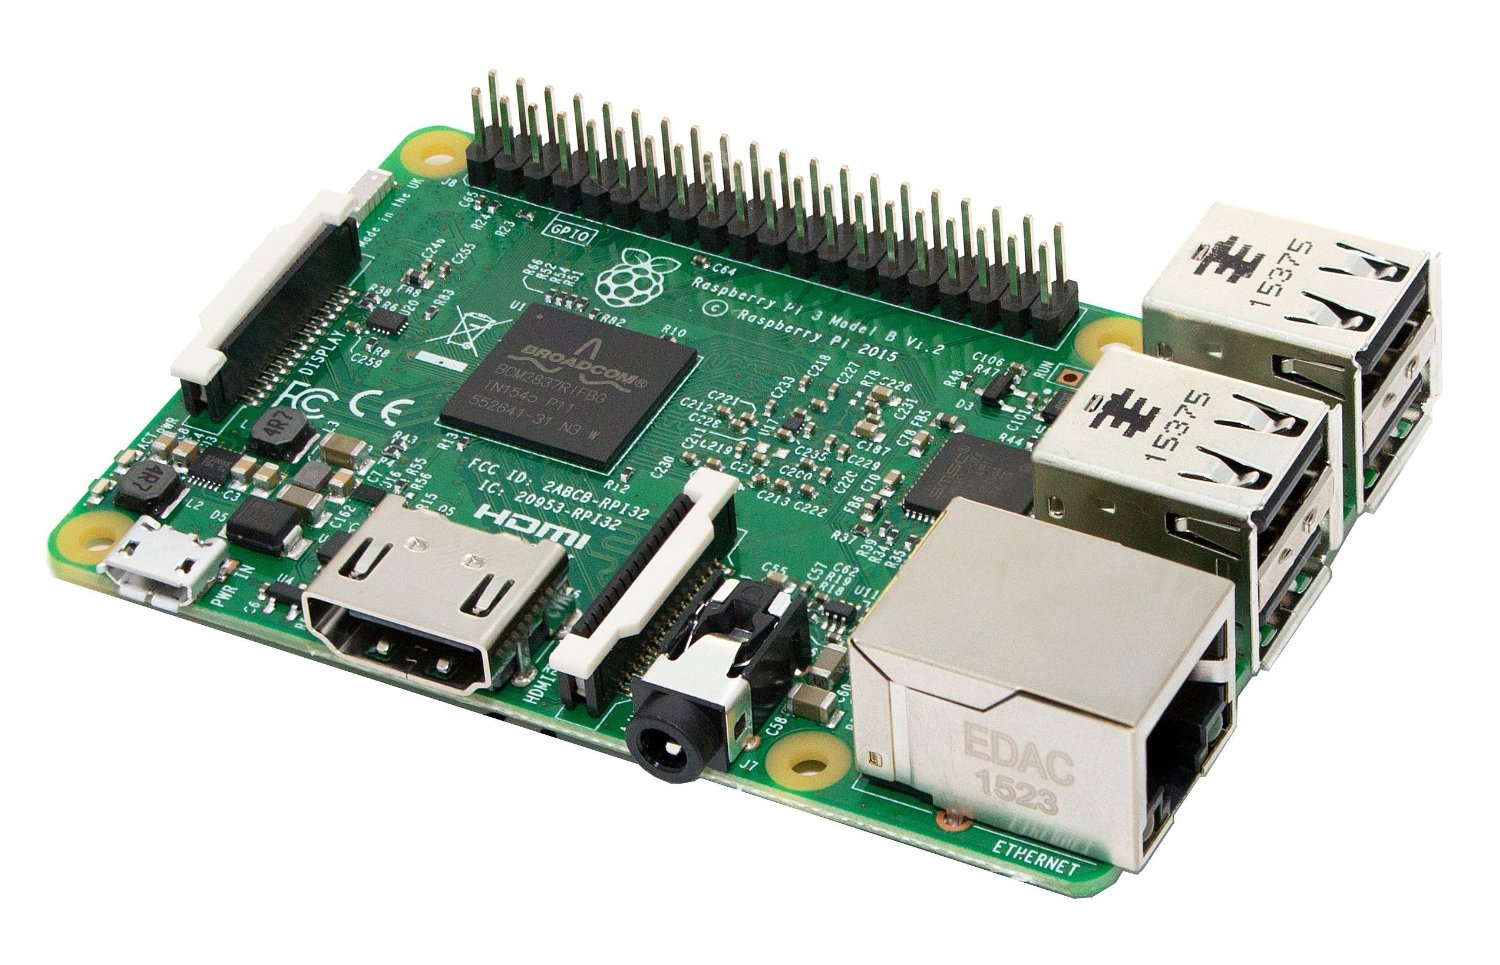
\includegraphics[width=9cm,height=5cm]{figure_v}
	\caption{Raspberry Pi 3 model B}
	\label{figure_v}
\end{figure}
\begin{center}
\begin{tabular}{ |l||p{12cm}|}
	\hline
	Processor      & Broadcom BCM2387 chipset. 1.2GHz Quad-Core ARM Cortex-A53 802.11 b/g/n Wireless LAN and Bluetooth 4.1 (Bluetooth Classic and LE)\\ \hline
	GPU               & Dual Core VideoCore IV® Multimedia Co-Processor. Provides Open GL ES 2.0, hardware-accelerated OpenVG, and 1080p30 H.264 high-profile decode. \\ \hline
	Memory          & 1GB LPDDR2  \\ \hline
	Operating System  & Boots from Micro SD card, running a version of the Linux operating system  \\ \hline
	Dimensions     & 85 x 56 x 17mm  \\ \hline
	Power             & Micro USB socket 5V1, 2.5A  \\ \hline
	Ethernet          & 10/100 BaseT Ethernet socket  \\ \hline
	Video Output   & HDMI (rev 1.3 \& 1.4 Composite RCA (PAL and NTSC)  \\ \hline
	Audio Output   & Audio Output 3.5mm jack, HDMI     \\ \hline
	USB                 & 4 x USB 2.0 Connector   \\ \hline
	GPIO Connector    & 40-pin 2.54 mm (100 mil) expansion header: 2x20 strip Providing 27 GPIO pins as well as +3.3 V, +5 V and GND supply lines \\ \hline
	Camera Connector  & 15-pin MIPI Camera Serial Interface (CSI-2) \\ \hline
	Display Connector & Display Serial Interface (DSI) 15 way flat flex cable connector with two data lanes and a clock lane    \\ \hline
	Memory Card       & Slot Push/pull Micro SDIO  \\ \hline
\end{tabular}
\end{center}


\subsection{NIMH battery}
We used a 5 volts NIMH battery to power up servo motors. With 1500 mAh capacity, ZagHexa is able to run for about 15 minutes.

\begin{figure}[H]
	\centering
	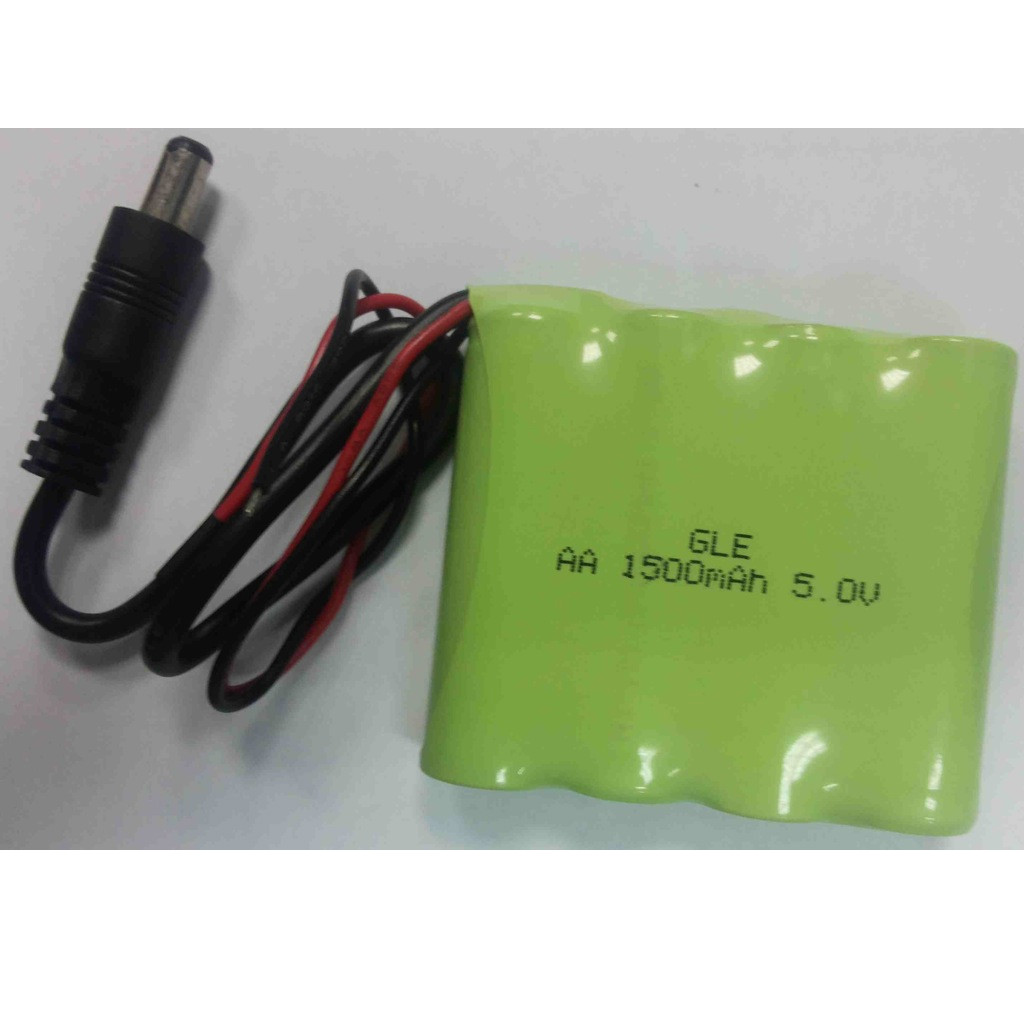
\includegraphics[width=8cm,height=5cm]{figure_w}
	\caption{5V NIMH battery}
	\label{figure_w}
\end{figure}

%%%%%%%%%%%%%%%%%%%%%%%%%%%%%%%%%%%%%%%%%%%%%%%%%%%%%%%%%%%%%%%%%%%%%%%%%%%%%%%

\setchapterpreamble[o]{%
    \dictum[Alan Turing, \textit{(British pioneering computer scientist, cryptanalyst,$\cdots$, and philosopher, 1912--1954)}]{%
        ``A computer would deserve to be called intelligent if it could deceive a human into believing that it was human.''}}

\chapter{Mechanical Design} \label{ch:mechanical}
%!TEX root = finalReport.tex
%!TEX encoding = UTF-8 Unicode
%==============================================================================

\section{Design Characteristics}
In the following section, the main design characteristics and modeling issues are discussed in order to show how the proposed design procedure can be implemented. It is worth mentioning also that other design characteristics exist and additional features can be considered for specific applications. Thus, the most remarkable design characteristics have been considered as examples for filling in the data in the cause and effect matrix.

\subsection{Robot Body Architecture}
There are two basic architectures of hexapod robots: rectangular and hexagonal as shown in \ref {figure a.png}. The first one has six legs distributed symmetrically along two sides,each side having three legs. The second haslegs distributed axi-symmetrically around the body, in a hexagonal or circular shape.

\begin{figure}[h]
	\centering
	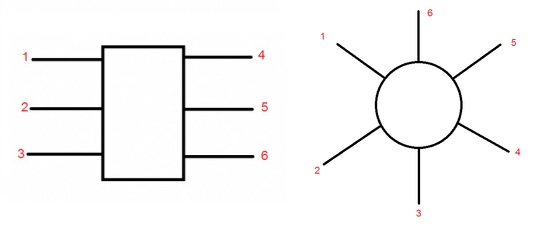
\includegraphics{figure_a}
	\caption{Basic architectures of hexapod robots}
	\label{figure a.png}
\end{figure}

Many references can be found in the literature on rectangular six-legged robots, they describe the longitudinal stability margin for rectangular hexapods. Also, the feasible walking gaits have been widely investigated and tested. Bilateral symmetry may be better suited than radial symmetry to move along a straight line. Rectangular architectures require a special gait for turning action; generally, they need four steps in order to realize a turning action. Hexagonal hexapod robots demonstrate better performances than rectangular robots for some aspects. As example hexagonal robots can have many kinds of gaits and can easily change direction—in fact true radial symmetry implies that all legs are equal and the body has no “front” or “rear”—there is thus no preferential directionfor the motion. It is proved that hexagonal hexapods can easily steerin all directions and that they have a longer stability margin. It isfound that hexagonal robots rotate and move in all directions at the same time,better than rectangular ones, by comparing stability margin and stroke in wave gait.It is proved theoretically that hexagonal hexapod robots have superior stability margin,stride and turning ability compared to rectangular robots.

\subsection{Kinematic Architectures of Legs}
Kinematics architecture depends on the factors related to the application in which the hexapod robot is required for, as for example the terrain form, the workspace and the payload. Literature shows that there is a number of different leg types currently employed for hexapod walking robots. All have advantages and disadvantages. \ref{figure b.png} shows a schematic classification of hexapod legs types.

\begin{figure}[h]
	\centering
	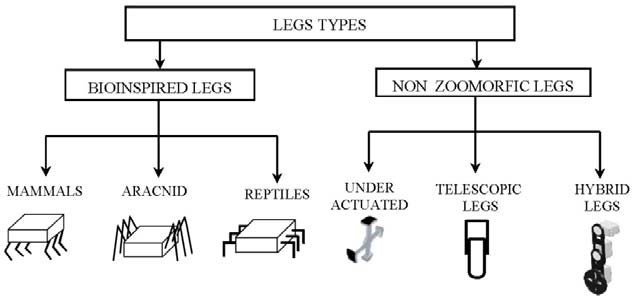
\includegraphics[width =0.85\textwidth]{figure_b}
	\caption{Classification of hexapod leg types}
	\label{figure b.png}
\end{figure}

At the first stage, one can choose between bio inspired and non-zoomorphic legs. Bio inspired leg configuration is motivated primarily by animal gait, such as reptiles, mammals or arachnid. The first one has legs and bodies for moving over rough and uneven terrains. The principal characteristic of the Reptilian type is that the legs are placed on both ends of the protruding body and knees to the side of the base. Mammals’ bodies are above the legs, which gives less support to the base and lower power consumption is needed to support the body, but it requires more stability than other types of animal. In Arachnid configuration, legs extremities are situated on both sides, sticking the knees at the top of the spider’s body. The orientation of the legs in respect to the body of the hexapod robot can be done with three configurations: frontal, sagittal or circular as shown in \ref{figure c.png}.
\begin{figure}[h]
	\centering
	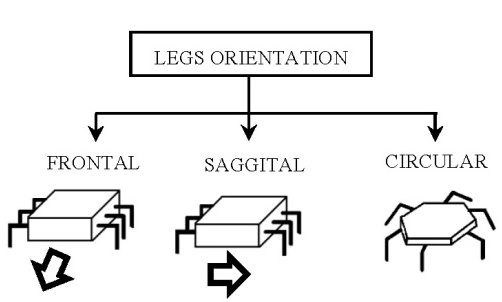
\includegraphics[width =0.75\textwidth]{figure_c}
	\caption{Hexapod leg configurations}
	\label{figure c.png}
\end{figure}

In the first one, the directions are perpendicular to the advancement of the legs’ position, unlike the sagittal, which moves parallel to the robot legs, while in the circular arrangement the legs are positioned radially to the body of the system allowing the mechanism to move in any direction. In the mammalian configuration, the legs are below the body and can place the knees in different positions depending on the application it requires, shown in figure (d). Non zoomorphic legs can be hybrids, telescopic or under-actuated, a solution named Roller-Walker is presented. The principle through which the robot propels itself during wheeled locomotion is the same as that of the skaters.

\begin{figure}[h]
	\centering
	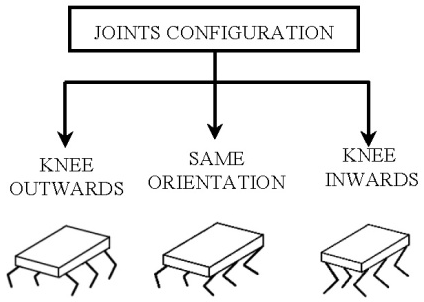
\includegraphics[width =0.75\textwidth]{figure_d}
	\caption{Joint configurations}
	\label{figure d.png}
\end{figure}

\subsection{Actuator Types}
Many kinds of actuators can be employed for operating hexapod walking robots. The majority of hexapods is actuated by electric rotating motors (Servo motors), as they are relatively cheap, easy to control and there are suitable technologies to store the energy.\\ 
Linear motors are able to generate considerable forces at very considerable speeds. However, these do not yet appear to have been utilized in many hexapods since they have a limited movable range to weight ratio. Pneumatics actuators have very low stiffness, inaccurate response, and low power to weight ratio. Pneumatics actuators, or air muscle, are able to offer a fast response time but they need an on-board air supply as bottles or compressors that are heavy pieces of equipment. Hydraulics actuators have high power/weight ratio; they are able to supply very high force, but suffer from the serious drawback of having to carry an engine to drive the pump. Hydraulics actuators are suitable for larger sized hexapod robots.\\
Unconventional actuators for hexapod robots can also be materials that can change shape through the direct application of electricity or a chemical agent. Ionic polymer-metal composites, for example, are materials that exhibit high strains under applied voltage differences allowing them to change from a sheet shape into curved shapes. Polyacrylonitrile is a form of artificial silk, classed as a gel polymer. It can respond fast, but the activation method is a change in pH, which requires the fibers to be housed in a watertight bag. Another class of materials that can change shape under the application of electricity is the Shape Memory Alloys (SMA), such as a nickel-titanium alloy that exhibits extreme contraction when heated.\\
Contraction rates are controlled by the heating and cooling; the major drawback resulting in slow response times and small operating forces. Thus, despite a great research interest and the building of some prototypes, the uses of SMA as hexapod actuators have been very limited. Present trends indicate that they are more suited to micro robots.

\subsection{Actuators Arrangements}
Typically, specific actuator arrangements are developed in order to obtain maximum leg workspace with a minimal kinematic structure. Several types of geometrical arrangements such as in \ref{figure_e} are recurrent in literature.
\begin{figure}[h]
	\centering
	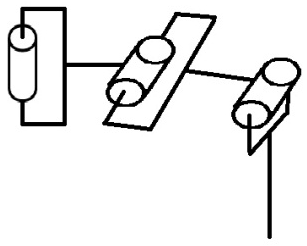
\includegraphics[width =0.5\textwidth]{figure_e}
	\caption{Three DoF solution}
	\label{figure_e}
\end{figure}

The design consists of links connected through knee joints. The walking motion is accomplished by controlling the angle of the links to position the feet. There are a number of different ways in which the joints can be actuated. Options include mounting the motor at the joint itself, or using a pulley and belt or lead screw \ref{figure_f} to set the angle of the knee using an actuator mounted near the base of the leg.
\begin{figure}[h]
	\centering
	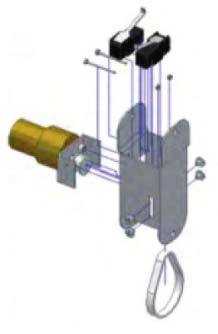
\includegraphics{figure_f}\qquad
    	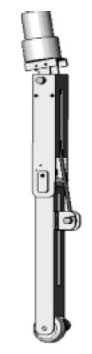
\includegraphics{figure_g}
	\caption{Pinion-belt arrangement (left) and Lead screw leg (right)}
	\label{figure_f}
\end{figure}


The major drawback of last design is the necessity to actuate remote joints. On the other hand, latching the actuator at the knee joint adds various dynamic effects to the leg which have to be compensated by the controller. This adds complexity to the control algorithms needed to move the leg.\\
It also requires more powerful motors at the hip joint to move the added mass of the leg. Remote actuation, in which the actuators are located at the base of the leg, eliminates some of these problems, at the cost of increasing the complexity of the mechanism. The coupling of the motion of the end effector relative to the actuators is another undesirable characteristic of this leg design.  Another potential leg design is modeled according to a typical mammalian leg with a four-bar linkage structure. The major drawback of this design is that the motions are highly coupled and the effective workspace is somewhat limited. Moreover, the entire weight of the robot is supported by the hip joint and they necessitate a powerful and expensive motor.

\section{Walking Gaits}
A gait is a sequence of leg motions coordinated with a sequence of body motions for moving the overall body of the robot in the desired direction and for orientation from one place to another. A gait is described as periodic when similar states of the same leg during successive strokes occur at the same interval for all legs. Periodic gaits are suitable for smooth terrain and they have been studied by several investigators. Figure 9 shows the scheme of some periodical hexapod gaits; white color indicates that the foot is in ground contact and the black color otherwise. Figure 9a reports the hexapod legs’ description.

\subsection{Tripod gait}
Tripod gait is a regular, periodic gait where the anterior and posterior legs on one side lift in time with the contralateral middle leg, forming alternating tripods. Thus, it is based on two groups of legs. During each step the first group of the legs is lifted and is rotated forward and is laid upon on the ground. Then the other group is lifted. Now both groups are moving, the first group backward, the second group forward and finally the second group is laid on the ground. It is obvious that both groups perform the same movement, but they are shifted by half a period. Tripod gait is very fast, but also very unstable. That is because at one moment half of the whole weight of the robot is only on one leg, which can lead to slip or even to fall. This is a gait suitable for high speed walking over relatively flat ground.

\subsection{Wave Gait}
Another gait is wave, which is the most stable gait, but also the slowest. Wave gait consists of a sequential adjustment of legs forward and only when all the legs are set to the new positions, the step is completed. In each phase of step maximally one leg is lifted up, which leads to high stability of this gait.

\subsection{Ripple Gait}
Ripple gait is inspired by insects. Each leg performs the same move – up, forward, down, backward.

\begin{figure}[h]
	\centering
	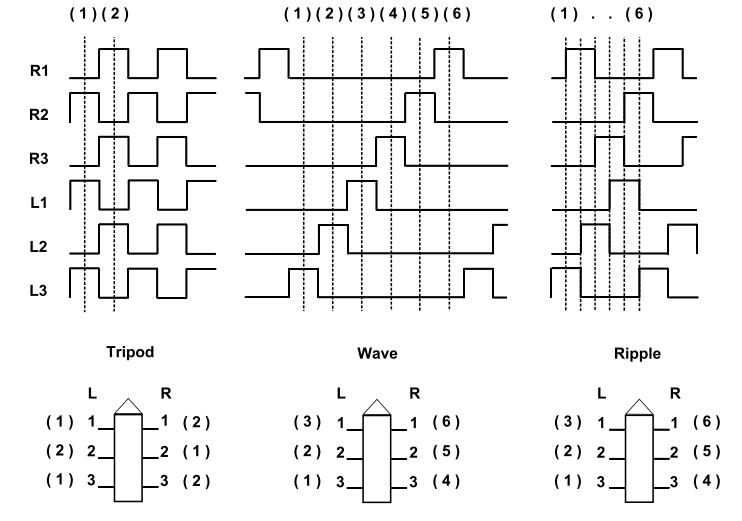
\includegraphics[width =0.8\textwidth]{figure_h}
	\caption{Gait diagram of hexapodal gaits}
	\label{figure h.png}
\end{figure}

\ref{figure h.png} shows the movement of each leg in time. A high value represents leg movement and low values means no movement. Tripod, wave and ripple gaits are shown in this figure. Tripod has two group of legs, all the legs in the same group move at once. In the wave gait only one leg is moving at any time. After all legs are set up to their new positions, step is completed. In the ripple gait all legs move the same way, but their moves are shifted. Leg moves partially overlap. In other words, the time when the first foot is lifted and begins to move forward, the second leg begins to lift up. In this way the robot cycles through all legs.

These are the most common gaits. Theoretical number of different gaits N can be calculated using equation: N = (2K - 1)!, where K is the number of the legs of the robot. Not all of them are usable for effective locomotion. For hexapod robot it is 11! = 39 916 800 possibilities of locomotion. The number is quite large, because this equation calculates all possible motions, like motion up and down, which of course doesn’t lead to an effective movement.

\section{Robot Kinematics}

\subsection{Robot body frame}
The origin of the robot base frame will be in the center of the body, structured with Z-axis pointing up, the X-axis positioning right and Y-axis pointing forwards with respect to the robot front side as depicted in \ref{Loc}.

\begin{figure}[h]
	\centering
	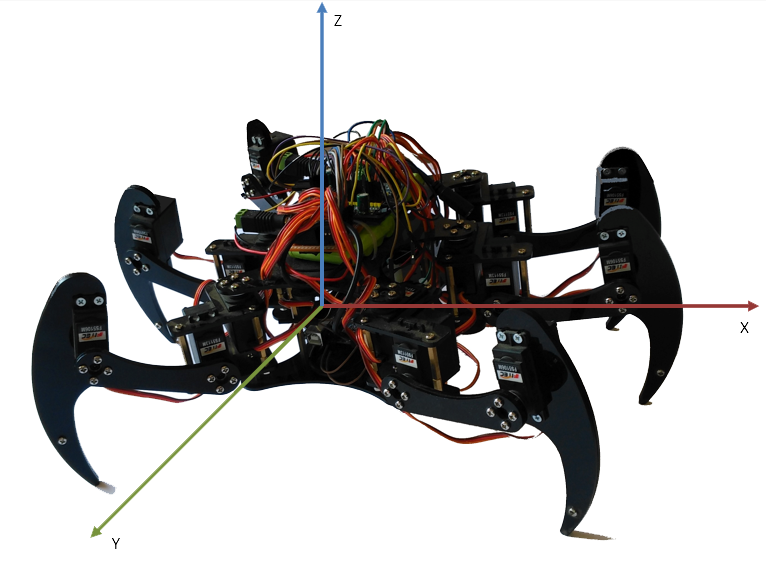
\includegraphics[width =0.8\textwidth]{Fig3}
	\caption{ Location of body frame relative to robot hardware.}
	\label{Loc}
\end{figure}

\subsection{Leg frames and notations}
The design of hexapod constitutes the kinematic configuration of a hexapod robot, with each leg acting as an independent serial manipulator with three degrees of freedom. Figure \ref{fig1} shows the actual prototype of our robot.

\begin{figure}[h]
	\centering
	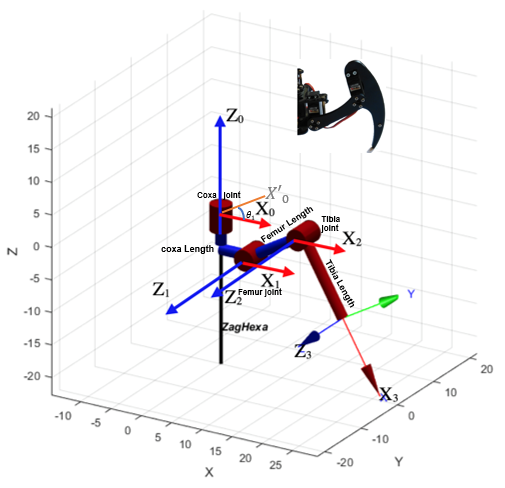
\includegraphics[width =.8\textwidth]{fream}
	\caption{  Final leg design (top right) and its notations, reference frames, joints and links.}
	\label{fream}
\end{figure}

The final leg design and its links and joints notations are given in \ref{fream}. The robot leg is made of links and joints as noted on \ref{leg}, different links of robot leg are called Femur, Tibia and Tarsus. As depicted in figure, the robot leg frame starts with link 0, which is the point where the leg is attached to the body, link 1, is Femur, link 2 is the Tibia and link 3 is Tarsus. The joints are located at the inner end of their respective link. Frames are attached to outer end of their respective links, this means that joint 2 rotates about the Z-axis of frame 1.

\begin{figure}[h]
	\centering
	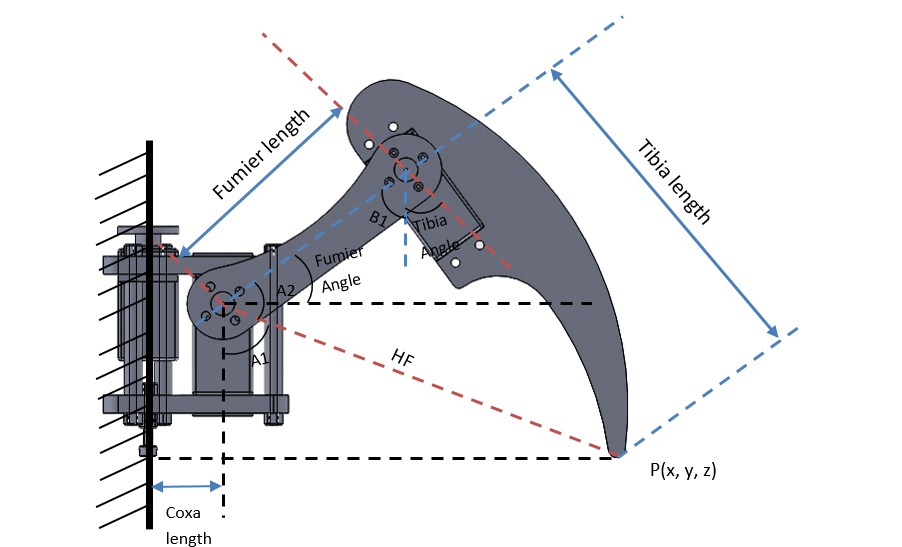
\includegraphics[width =.8\textwidth]{Fig7}
	\caption{  Final leg design (top right) and its notations, reference frames, joints and links.}
	\label{leg}
\end{figure}

\subsection{Robot Leg Parameters}
Following the well-known Denavit-Hartenberg (DH) notation, coordinate frames for the robot leg are assigned. The assigned frames are shown in \ref{leg}. In figure, the body {b} and the zeroth {0} reference frames are attached to the stationary robot body. Therefore, they can be both considered as inertial frames. The axes of the body frame are arranged to be in accord with the actual robot-body orientation. The DH link parameters based on \ref{leg} are given in Table II.\\

The resulting homogeneous transformation matrices between the body and the zeroth frame and between the sequential link frames are given in (1).  In the formulas, the variables represented by $a$ stand for the length of the $i^{th}$ link (namely, the length of the portion of the link between the origins of $(i-1) th and i^{th}$ reference frames). The variables represented by $\theta_{ij}$ mean the sum of the $i^{th}$ and $j^{th}$ joint angles $(\theta_{ij}=\theta_i+\theta_j)$. C and S are for cos(.) and sin(.) functions, respectively.  The exact values of these variables corresponding to ZagHexa robot are: 
$\psi = 45^\circ, a_1= 5cm, a_2= 9cm, a_3= 18cm$
\begin{center}
\begin{tabular}{|c||c|c|c|c|}
	\hline
	Joint & $\theta_i$ & $\alpha_i$ & $a_i$ & $d_i$ \\ \hline
	1&		$\theta_1$ & $\pi/2$	& $a_1$ & 0 \\ \hline
	2&		$A_2$ & 0			& $a_2$ & 0 \\ \hline
	3&		$B_1$ & 0			& $a_3$ & 0 \\ \hline
\end{tabular}
\end{center}

Homogeneous matrices are used in derivation of positional relations between the successive frames.  In (3) the leg tip point position with respect to the body frame is given. The rotation matrices between the frames are given in (2). These rotation matrices are used in vector equations, especially while deriving the dynamic equations.
\begin{center}

\[
H^{(b,0)}=
\begin{bmatrix}
0 & \cos(\psi) & \sin(\psi) & 0 \\
-1&		0	   & 		0 	& 0\\
0 & -\sin(\psi)& \cos(\psi) & 0 \\
0 &		0	   & 		0 	& 1
\end{bmatrix}
\]
\end{center}

\begin{equation}
H^{(K-1,K)} =
\begin{bmatrix}
\cos\theta_k &-\cos\alpha_k\sin\theta_k &\sin\alpha_k\sin\theta_k &a_k\cos\theta_k\\
\sin\theta_k &\cos\alpha_k\cos\theta_k &-\sin\alpha_k\cos\theta_k &a_k\sin\theta_k\\
0 &\sin\alpha_k &\cos\alpha_k &d_k \\ 
0 &0 &0 &1
\end{bmatrix}
\end{equation}

\begin{align*}
H^{(0,3)} = H^{(0,1)} H^{(1,2)} H^{(2,3)} H^{(b,3)}= H^{(b,0)} H^{(0,3)}
\end{align*}

\begin{center}
	
	\[
	C^{(b,0)}=
	\begin{bmatrix}
	0 & \cos(\psi) & \sin(\psi) \\
	-1&		0	   & 		0 	\\
	0 & -\sin(\psi)& \cos(\psi) \\

	\end{bmatrix}
	\]
\end{center}

\begin{equation}
C^{(K-1,K)} =
\begin{bmatrix}
\cos\theta_k &-\cos\alpha_k\sin\theta_k &\sin\alpha_k\sin\theta_k \\
\sin\theta_k &\cos\alpha_k\cos\theta_k &-\sin\alpha_k\cos\theta_k \\
0 &\sin\alpha_k &\cos\alpha_k \\ 
\end{bmatrix}
\end{equation}
\begin{equation}
P_e^{(K-1,K)} (\theta) =
\begin{bmatrix}
C\psi(a_1S\theta_1+a_2S\theta_1C\theta_2+a_3S\theta_1C\theta{23})+S\psi(a_2S\theta_2+a_3\theta_{23}) \\
-(a_1C\theta_1+a_2C\theta_1C\theta_2+a_3C\theta_1C\theta_{23})  \\
-S\psi(a_1S\theta_1+a_2S\theta_1C\theta_2+a_3S\theta_1C\theta{23})+C\psi(a_2S\theta_2+a_3\theta_{23}) \\
\end{bmatrix}
\end{equation}
To derive the dynamic equations, first the inertia matrices of the links should be determined. Since the $k^{th}$ reference frame is stationary with respect to the $k^{th}$ link, the inertia tensor of the $k^{th}$ link around its center of mass appears to be a constant matrix with respect to the $k^{th}$ reference frame, as in (4). The values used in these formulations belong to the Hexapod robot. The resulting matrices for each link are in the form of (5).
\begin{equation}
\{J_K\}^{(K)} = J_K^{(K)} = J_K
\end{equation}
\begin{equation}
J_K = \begin{bmatrix}
J_{K1} & 0      & 0 \\
0      & J_{K2} & 0 	\\
0      & 0      & J_{K3} 
\end{bmatrix}
\end{equation}

\subsection{Inverse kinematics}
The forward kinematics (FK) is a simple equation used to calculate the position of the end effectors for the leg in the robot base frame, by injecting values of each joint angle. But the reverse operation, namely inverse kinematics (IK), is more complex. IK is employed to find all the joint angles given the position of the end effectors. In general, solving the IK equations can be a bit of a challenge. Some positions cannot be reached at all, as the physical system is unable to get there, and some end effectors positions can have more than one solution, and not all of them are desirable.
\begin{figure}[h]
    \centering
    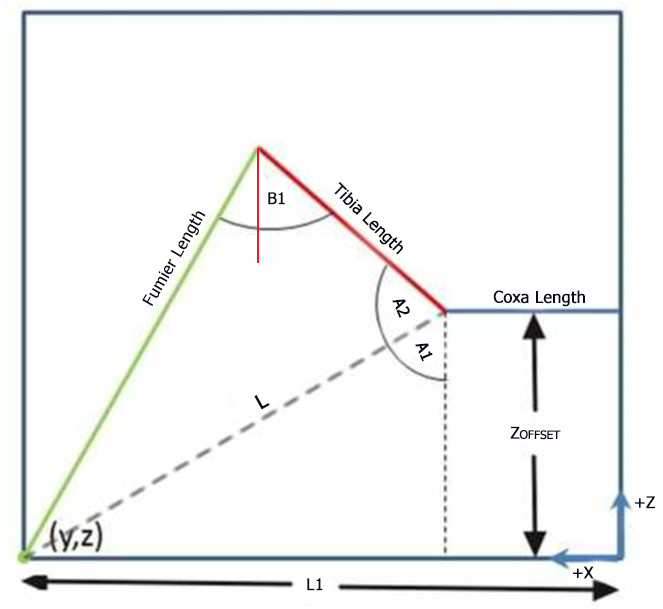
\includegraphics[width =.55\textwidth]{Fig8.png}
    \caption{ Illustration of the 2D triangle with vertices in the coxa, the femur, and tibia link from origin.}
    \label{fig8}
\end{figure}
We solve the IK problem for each leg separately, as this makes it possible to solve it geometrically, by setting up some constrains. The first constraint for solving the IK equations due the fact that all robot joints allow rotation about one axis only. The second constraint is that the Femur, Tibia joints always rotate on parallel axes. The third set of constraints arises from the physical limitations for each joint, giving us some angular interval for each joint in which the servos can actually rotate the link. In \ref{leg}, the angles of movement are shown.
First, the coxa angle can be found directly by knowing the end effectors position then simply using $atan2(y,x)$ to calculate it.  \ref{eq:invS} through \ref{eq:invE} are used to find the individual joint angles.
\begin{align}
    \frac{x}{y} & =\tan (\gamma)\to \gamma =\tan ^{-1}\frac{x}{y} \label{eq:invS}\\
    L              & = \sqrt{Z_{offset}^{2}+(L_{1}+\cos (A_1 + A_2))^{2}}\\
    A_{1}        & = \cos ^{-1}(\frac{Z_{offset}}{L})\\
    Tibia^{2}  & =Femar^{2}+L^{2}-2(Femar)(L)\cos \alpha _{2} \\
    A_{2} & =\cos^{-1}(\frac{Tibia^{2}-Femar^{2}-L^{2}}{-2(Femar)(L)}) \\
    A & =A_{1} + A_{2}\\
    A & = \cos ^{-1}\left(\frac{Z_{offset}}{L})+\cos ^{-1}(\frac{Tibia^{2}-Femar^{2}-L^{2}}{-2(Femar)(L)}\right) \\
    B & = \cos^{-1}\left(\frac{L^{2}-Femar^{2}-Tibia^{2}}{-2(Femar)(Tibia)}\right) \label{eq:invE}
\end{align}


\setchapterpreamble[o]{%
	\dictum[Richard P. Feynman, \textit{(American theoretical physicist, 1918--1988)}]{%
		``It doesn't matter how beautiful your theory is, it doesn't matter how smart you are. If it doesn't agree with experiment, it's wrong.''}}
\chapter{Experiments and Simulation} \label{ch:simulation}
%!TEX root = finalReport.tex
%!TEX encoding = UTF-8 Unicode
%==============================================================================
%\section{Introduction}
Programming directly on a real robot gives us good feedback and it is more impressive
than simulations, but not everybody has possible access to real robots. For this reason,
we have programs that simulate the physical world.\\
The first phase of robot manufacturing is its design and modeling. We can design and model the 
robot using CAD tools such as Solid Works, Blender, and so on. One of the main purposes 
of modeling robot is simulation. The robotic simulation tool can check the critical flaws in the robot design and can confirm the 
working of the robot before it goes to the manufacturing phase.

The virtual robot model must have all the characteristics of real hardware, the shape of robot 
may or may not look like the actual robot but it must be an abstract, which has all the physical 
characteristics of the actual robot. 

If we are planning to create the 3D model of the robot and simulate using ROS, you need to learn about some ROS packages which helps in robot designing. ROS has a standard meta package for designing, and creating robot models called robot model, which consists of a set of packages called urdf, robot state publisher and so on.  These packages help us create the 3D robot model description with the exact characteristics of the 
real hardware.

In this chapter, we will cover the following topics:
\begin{enumerate}
\item ROS packages for robot modeling
\item  Understanding robot modeling using URDF
\item  Creating our URDF model
\item  Watching the 3d model in RVIZ
\item  Making our robot movable
\end{enumerate}

\section{ROS packages for robot modeling}
The way ROS uses the 3D model of a robot or its parts, to simulate them. ROS provides some good packages that can be used to build 3D robot models.\\ In this
section, we will discuss some of the important ROS packages that are commonly used to
build robot models:
\\\\\textbf{robot model}: ROS has a meta package called robot model, which contains important 
packages that 
help build the 3D robot models. We can see all the important packages inside this meta-
package:
\\\\\textbf{URDF}: One of the important packages inside the robot model meta package is urdf. The 
URDF package contains a C++ parser for the Unified Robot Description Format (URDF),
which is an XML file to represent a robot model.
\\\\ We can define a robot model, sensors, and a working environment using URDF and 
can parse it using URDF parsers.
\\We can only describe a robot in URDF that has a tree-like 
structure in its links, that is, the robot will have rigid links and will be connected 
using joints. Flexible links can't be represented using URDF.
\\ The URDF is composed using special XML tags and we can parse these XML tags using 
parser programs for further processing. We can work on URDF modeling in the upcoming 
sections.
\\\\\textbf{joint state publisher}: This tool is very useful while designing robot 
models using URDF.
\\This package contains a node called joint state publisher, which reads the robot 
model description, finds all joints, and publishes joint values to all non fixed 
joints 
using GUI sliders. 
\\The user can interact with each robot joint using this tool and can visualize using 
RViz.
\\While designing URDF, the user can verify the rotation and translation of each 
joint using this tool. 
\\\\\textbf{kdl parser}: Kinematic and Dynamics Library (KDL) is an ROS package that 
contains parser tools to build a KDL tree from the URDF representation. The kinematic 
tree can be used to publish the joint states and also to forward and inverse 
kinematics of the robot.
\\\\\textbf{robot state publisher}: This package reads the current robot joint states 
and publishes 
the 3D poses of each robot link using the kinematics tree build from the URDF. The 3D 
pose of the robot is published as ROS tf (transform). ROS tf publishes the 
relationship 
between coordinates frames of a robot.
\\\\\textbf{xacro}: Xacro stands for (XML Macros) and we can define how xacro is equal 
to URDF plus add-ons. It contains some add-ons to make URDF shorter, readable, and can 
be used for building complex robot descriptions. We can convert xacro to URDF at any 
time using some ROS tools. We will see more about xacro and its usage in the upcoming 
sections.

\section{Understanding robot modeling using URDF}

We have discussed the urdf package. In this section, we will look further at the URDF XML tags, which help to model the robot. We have to create a file and write the relationship between each link and joint in the robot and save the file with the .urdf extension.
\\The URDF can represent the kinematic and dynamic description of the robot, visual representation of the robot, and the collision model of the robot.
\\\\The following tags are the commonly used URDF tags to compose a URDF robot model:
\\ \textbf{link}: The link tag represents a single link of a robot. Using this tag, we can model a robot link and its properties. The modeling includes size, shape, color, and can even import a 3D mesh to represent the robot link. We can also provide dynamic properties of the link such as inertial matrix and collision properties.
\\
The syntax is as follows:
\begin{lstlisting}[language=XML]
<link name="<name of the link>">
    <inertial>...........</inertial>
    <visual> ............</visual>
    <collision>..........</collision>
</link>
\end{lstlisting}

The following is a representation of a single link. The Visual section represents 
the real link of the robot, and the area surrounding the real link is the Collision 
section. The Collision section encapsulates the real link to detect collision before 
hitting the real link.
\begin{figure}[h]
	\centering
	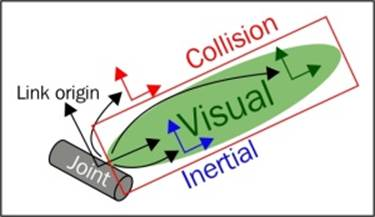
\includegraphics[width=0.7\linewidth]{s1}
	\caption{Visualization of a URDF link}
	\label{fig:s1}
\end{figure}
\textbf{joint}: The joint tag represents a robot joint. We can specify the kinematics and dynamics of the joint and also set the limits of the joint movement and its velocity. The joint tag supports the different types of joints such as revolute, continuous, prismatic,fixed, floating, and planar.

The syntax is as follows:
\begin{lstlisting}[language=XML]
<joint name="<name of the joint>">
  <parent link="link1"/>
  <child link="link2"/>
  <calibration .... />
  <dynamics damping ..../>
  <limit effort .... />
</joint>
\end{lstlisting}
A URDF joint is formed between two links; the first is called the Parent link and the second is the Child link. The following is an illustration of a joint and its link:\\
\begin{figure}[h]
	\centering
	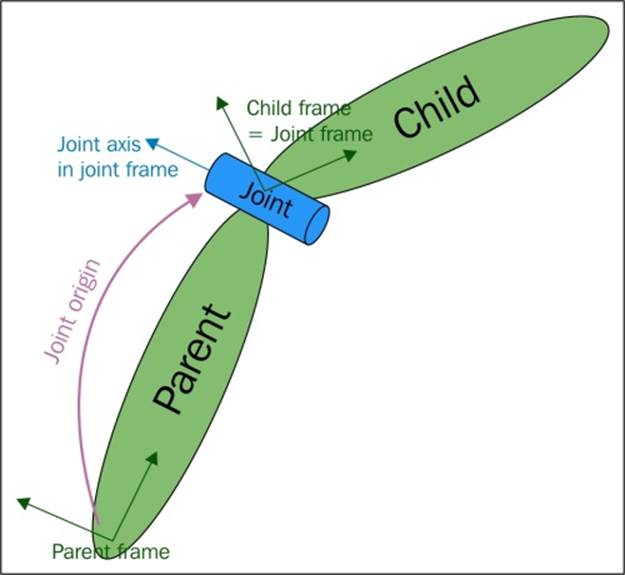
\includegraphics[width=0.6\linewidth]{s2}
	\caption{Visualization of a URDF joint}
	\label{fig:s2}
\end{figure}
\textbf{robot}: This tag encapsulates the entire robot model that can be represented using URDF. Inside the robot tag, we can define the name of the robot, the links, and the joints of the robot.
The syntax is as follows:
\begin{lstlisting}[language=XML]
<robot name="<name of the robot>"
  <link>  ..... </link>
  <link> ...... </link>
  <joint> ..... </joint>
  <joint> ..... </joint>
</robot>
\end{lstlisting}
A robot model consists of connected links and joints. Here is a visualization of the robot model:
\begin{figure}[h]
	\centering
	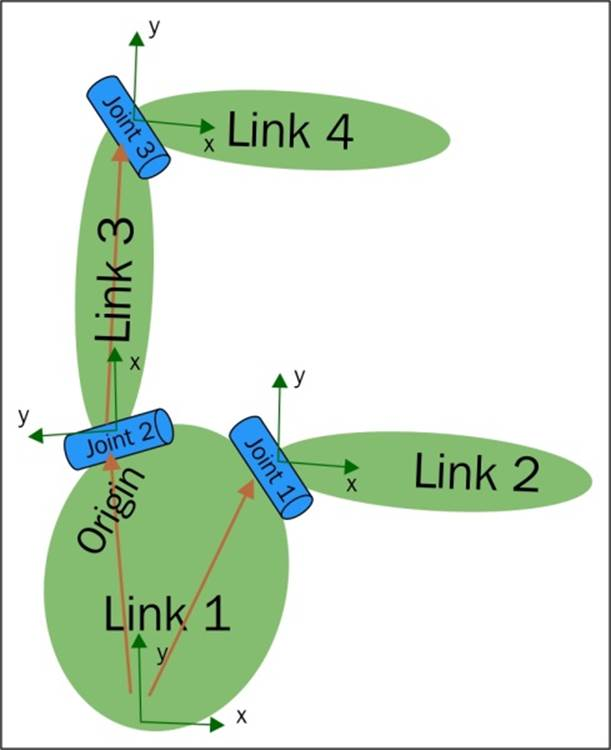
\includegraphics[width=0.7\linewidth]{s3}
	\caption{Visualization of a robot model having joints and links}
	\label{fig:s3}
\end{figure}

\section{Creating our URDF model}
To start first we create the urdf file, let's call it\textit{ zaghexasim.urdf} and put in
the following code; this URDF code is based on XML.As you will see in the code, there are two principal fields that describe the geometry of a robot: links and joints.\\
the first link has the name base link; this name must be unique to the file\\
\begin{lstlisting}[language=XML]
<?xml version="1.0" ?>
<robot name="zaghexa" xmlns:xacro="http://ros.org/wiki/xacro">
 <!-- Build the body frame -->
<link name="base_link"/>
<joint name="base_joint" type="fixed">
<parent link="base_link"/>
<child link="box"/>
<origin rpy="0 0 0" xyz="0 0 0"/>
</joint>
<link name="box">
<visual>
<origin rpy="0 0 0" xyz="0 0 0"/>
<geometry>
<mesh filename="package://zaghexa_sim/meshes/box.STL"/>
</geometry>
<material name="grey">
<color rgba="0.5 0.5 0.5 1"/>
</material>
</visual>
</link>
\end{lstlisting}
In the joint field we define the name which must be unique as well also we define 
the type of joint(fixed,revolute,continous,floating or planar) the parent, and the child.\\
in our case tibia,femur and leg centre joint are the children of base link which is fixed but all of other joints are revolute.\\
\textbf{this is a sample of one leg and how does it build}\\
\begin{lstlisting}[language=XML]
<!-- Joint properties -->
<!-- Leg macros -->
<!-- Build robot model -->
<joint name="leg_center_joint_r1" type="fixed">
<origin rpy="0 0 0" xyz="0.087598 -0.050575 0"/>
<parent link="box"/>
<child link="leg_center_r1"/>
</joint>
<link name="leg_center_r1"/>
<joint name="coxa_joint_r1" type="revolute">
<origin rpy="0 0 -1.0471975512" xyz="0 0 0"/>
<parent link="leg_center_r1"/>
<child link="coxa_r1"/>
<axis xyz="0 0 -1"/>
<limit effort="10000" lower="-1.5" upper="1.5" velocity="100"/>
</joint>
<link name="coxa_r1">
<visual>
<origin rpy="0 0 0" xyz="0 0 0"/>
<geometry>
<mesh filename="package://zaghexa_sim/meshes/coxa_r.STL"/>
</geometry>
<material name="">
<color rgba="0.7 0.7 0 1"/>
</material>
</visual>
</link>
<joint name="femur_joint_r1" type="revolute">
<origin rpy="-1.57079632679 0 0" xyz="0.0294 0 0"/>
<parent link="coxa_r1"/>
<child link="zaghexa"/>
<axis xyz="0 0 -1"/>
<limit effort="10000" lower="-1.5" upper="1.5" velocity="100"/>
</joint>
<link name="zaghexa">
<visual>
<origin rpy="0 0 0" xyz="0 0 0"/>
<geometry>
<mesh filename="package://zaghexa_sim/meshes/femur_r.STL"/>
</geometry>
<material name="">
<color rgba="0 0.7 0.7 1"/>
</material>
</visual>
</link>
<joint name="tibia_joint_r1" type="revolute">
<origin rpy="3.14159265359 0 1.57079632679" xyz="0.08 0 0"/>
<parent link="zaghexa"/>
<child link="tibia_r1"/>
<axis xyz="0 0 1"/>
<limit effort="10000" lower="-1.5" upper="1.5" velocity="100"/>
</joint>
<link name="tibia_r1">
\end{lstlisting}
\textbf{You can check the syntax of the urdf whether we have errors, we can use:
check urdf command tool:}
\begin{lstlisting}[language=terCmd]
$ rosrun urdf_parser check_urdf zaghexa_sim.urdf
\end{lstlisting}

If you want to see it graphically, you can use the urdf to graphiz command tool
\begin{lstlisting}[language=terCmd]
$ rosrun urdf_parser urdf_to_graphiz "`rospack find zaghexa_sim`/urdf/zaghexa_sim.urdf"
\end{lstlisting}
\textbf{The following is what you will receive as output:}
\begin{figure}[hbt]
    \centering
    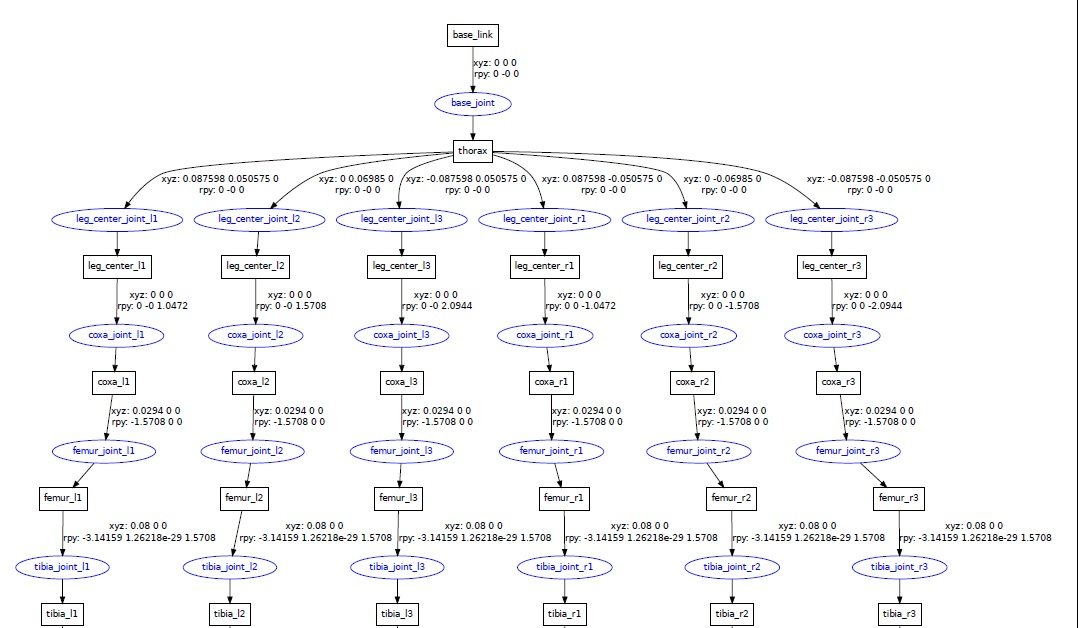
\includegraphics[width=\linewidth, height=0.5\textheight]{s4}
    \caption{output of urdf to graphics}
    \label{figure :s4}
\end{figure}

\section{Watching the 3D model in RVIZ}
Now that we have the model of our robot, we can use it on rviz to watch it in 3D
and see the movements of the joints.\\
We will create the display.launch file in zaghexa-sim/launch folder,
and put the following code in it:
\begin{lstlisting}[language=XML]
	<launch>
	<arg
	name="model" />
	<arg
	name="gui"
	default="True" />
	<param
	name="robot_description"
	command="$(find xacro)/xacro.py '$(find zaghexa_sim)/models/zaghexa_model.xacro'" />
	<param
	name="use_gui"
	value="$(arg gui)" />
	<param
	name="rate"
	value="25" />
	<rosparam param="source_list">
	[leg_joints_states]
	</rosparam>
	<node
	name="joint_state_publisher"
	pkg="joint_state_publisher"
	type="joint_state_publisher" />
	<node
	name="robot_state_publisher"
	pkg="robot_state_publisher"
	type="state_publisher" />
	<node
	name="rviz"
	pkg="rviz"
	type="rviz"
	args="-d $(find zaghexa_sim)/urdf.rviz" />
	</launch>
\end{lstlisting}	
\textbf{We will launch it with the following command:}
\begin{lstlisting}[language=terCmd]
$ roslaunch zaghexa_sim display_model.launch model:="`rospack find zaghexa_sim`/urdf/zaghexa_sim.urdf"
\end{lstlisting}

\textbf{if every thing is fine and you have no errors, it will load RVIZ and you will see:}
\begin{figure}[h]
	\centering
	\includegraphics[width=\linewidth, height=0.4\textheight]{s5}
	\caption{output of urdf to graphics}
	\label{figure :s5}
\end{figure}

\section{Making our robot movable}
\textbf{A good way of testing whether or not the axis and limits of the joints are fine by running rviz with joint state publisher GUI}
\begin{lstlisting}[language=terCmd]
$ roslaunch zaghexa_sim display.launch model:="`rospack find zaghexa_sim`/urdf/zaghexa_sim.urdf" gui:=true
\end{lstlisting}


\textbf{you will see a GUI with some sliders each of them controls one joint of the 18 joints so we have 18 sliders:}
%\begin{figure}[h]
%	\centering
%	\includegraphics[height=0.3\textheight]{s6}
%	\caption{Joint state publisher GUI}
%	\label{fig:s6}
%\end{figure}
\\\textbf{In the next figures you will see the effect of changing sliders values to the joints angles and positions}
\begin{figure}[h]
	\centering
	\includegraphics[width=\textwidth]{s7}
	\caption{Joint state publisher GUI with its control sliders and their effect on the robot }
	\label{fig:s7}
\end{figure}
\begin{figure}[htb]
	\centering
	\includegraphics[width=0.6\textwidth]{simViews}
    	\caption{Different views of the robot}
%	\caption{top view of the robot}
%	\label{fig:s8}
%	\includegraphics[height=0.3\textheight]{s9}
%	\caption{Different views of the robot}
%	\label{fig:s9}
%	\includegraphics[height=0.3\textheight]{s10}
%	\caption{Different views of the robot}
%	\label{fig:s10}
\end{figure}
%%%%%%%%%%%%%%%%%%%%%%%%%%%%%%%%%%%%%%%%%%%%%%%%%%%%%%%%%%%%%%%%%%%%%%%%%%%%%%%

%%%%%%%%%%%%%%%%%%%%%%%%%%%%%%%%%%%%%%%%%%%%%%%%%%%%%%%%%%%%%%%%%%%%%%%%%%%%%%%
\setchapterpreamble[o]{\dictum[George Henry Lewes, \textit{( English philosopher and critic of literature, 1817--1878)}]{The true function of philosophy is to educate us in the principles of reasoning and not to put an end to further reasoning by the introduction of fixed conclusions.}}
\chapter{Conclusions and Future Outlook} \label{ch:conclusion}
This paper presents a system description and the main aspects related to the design, construction, and implementation of six-leg robot named ZagHexa. The robot is a legged robot for search and rescue missions. It benefits form the reliability of its legged locomotion with the flexibility and versatility required to operate in different types of surface. The robot was constructed and tested to walk using tripod, wave and ripple gaits, can rotate and it is equipped with different sensors.

The robot was tested on different surfaces and in rugged terrain. The repeatability of the robot movement as well as the sensor system was also tested.	 These features are mainly achieved due to its original movement that make it deal with different surfaces. Additionally, its shape and weight give it more stability, and its ability to continue with its moving and sensing capabilities after collisions or even small falls. \\ 
However, more tests and experiments to improve and validate the design and sensor performance are to be carried out to optimize the system performance.
Finally, we are working on tackling some issues should to have fully autonomous operation and integration into a heterogeneous system. To make the integration of ZagHexa into different missions easier, an effort is being carried to provide it with a standard connectivity over the ROS framework.
%\input{chapters/futureWork}
%%%%%%%%%%%%%%%%%%%%%%%%%%%%%%%%%%%%%%%%%%%%%%%%%%%%%%%%%%%%%%%%%%%%%%%%%%%%%%%

\appendix
\renewcommand*\chapterformat{\color{blue}{Appendix \thechapter}\vspace{-0.6cm}}%\autodot
\chapter{This is My Appendix Title}\label{ch:cameraModel}
%%\input{chapters/appCameraModel}
%%%%%%%%%%%%%%%%%%%%%%%%%%%%%%%%%%%%%%%%%%%%%%%%%%%%%%%%%%%%%%%%%%%%%%%%%%%%%%%

\backmatter %------------------------------------------------------------------
\cleardoublepage{}
\renewcommand{\nomname}{List of Symbols and Abbreviations}
\markboth{\nomname}{\nomname}\printnomenclature{}
%\nocite{*}
\bibliographystyle{apalike}
%\include{myReferences}
\bibliography{myReferences}
%\cleardoublepage{}
%\printindex{} %\cleardoublepage{}
\end{document}